\documentclass[12pt, a4paper]{article}

% ─── Packages ─────────────────────────────────────────────
\usepackage[utf8]{inputenc}
\usepackage[T1]{fontenc}
\usepackage[margin=2.5cm]{geometry}
\usepackage{CJKutf8}
\usepackage{amsmath, amssymb, amsthm}
\usepackage{graphicx}
\usepackage{float}
\usepackage{booktabs}
\usepackage[hidelinks]{hyperref}
\usepackage{caption}
\usepackage{subcaption}
\usepackage{enumitem}
\usepackage{xcolor}
\usepackage{listings}
\usepackage{fancyhdr}

% ─── Paths ────────────────────────────────────────────────
\graphicspath{{figures/}}

% ─── Header/Footer ───────────────────────────────────────
\pagestyle{fancy}
\fancyhf{}
\fancyhead[L]{Random Walk}
\fancyhead[R]{2026}
\fancyfoot[C]{\thepage}

% ─── Code listing style ──────────────────────────────────
\lstset{
  basicstyle=\ttfamily\small,
  breaklines=true,
  frame=single,
  tabsize=4,
}

% ─── Title ────────────────────────────────────────────────

\begin{document}
\begin{CJK}{UTF8}{bsmi}  % bsmi = 明體 (macOS built-in)

\title{\textbf{Random Walk 模擬與分析} \\[0.5em]
       \large 機率模型及數據科學 2026 作業}
\author{廖子閔 \\[0.5em] 
        \small 專案開源網址：\url{https://github.com/killin0415/RandomWalkSimulation}}
\date{\today}

\maketitle
\tableofcontents
\newpage

% ╔═══════════════════════════════════════════════════════════╗
% ║  1. 簡介                                                  ║
% ╚═══════════════════════════════════════════════════════════╝
\section{簡介}

本報告旨在透過數值模擬研究 random walk 在 $D = 1, 2, 3, 4$ 維空間中的統計性質。
模擬程式以 C++ 實作，利用 OpenMP 進行平行化加速。

隨機行走的定義如下：在 $D$ 維空間中，粒子在每個 time step，
各維度獨立地以等機率 $\frac{1}{2}$ 移動 $+1$ 或 $-1$：
\begin{equation}
  x_d^{(i+1)} = x_d^{(i)} \pm 1, \quad d = 1, 2, \ldots, D
\end{equation}

對每個維度 $D \in \{1, 2, 3, 4\}$ 和步數 $n \in \{10^2, 10^3, 10^4, 10^5, 10^6\}$，
我們各執行 1000 次獨立的 random walk，並記錄以下統計量：
\begin{itemize}[nosep]
  \item 最終位置的 L1-norm 和 L2-norm 距離分佈
  \item 各 section（象限）的停留時間比例
  \item 回到原點（return to origin）的分佈
  \item（1D 限定）$m/n$ 分佈，與 arcsine law 的比較
\end{itemize}

% ╔═══════════════════════════════════════════════════════════╗
% ║  2. 模擬方法                                              ║
% ╚═══════════════════════════════════════════════════════════╝
\section{模擬方法}

\subsection{演算法}

模擬的核心演算法如下：
\begin{enumerate}[nosep]
  \item 初始化粒子位置為原點 $\mathbf{x}^{(0)} = \mathbf{0}$
  \item 對每個 time step $i = 1, 2, \ldots, n$：
    \begin{enumerate}
      \item 對每個維度 $d$，產生一個均勻隨機 bit，決定 $\Delta x_d = +1$ 或 $-1$
      \item 更新位置 $x_d^{(i)} = x_d^{(i-1)} + \Delta x_d$
      \item 記錄當前位置所屬的 section
      \item 檢查是否回到原點
    \end{enumerate}
  \item 記錄最終位置並計算 L1、L2 距離
\end{enumerate}

\subsection{隨機數生成}

使用 C++ 標準庫的 \texttt{std::mt19937\_64}（Mersenne Twister 64-bit）作為
pseudo-random number generator (PRNG)。每組行走使用確定性的 seed，
確保實驗的 reproducibility。

\subsection{平行化}

利用 OpenMP 將 1000 次行走分配至多個 thread，每個 thread 使用獨立的 PRNG instance，
避免 data race 並確保結果的正確性。

\subsection{機率密度估計}

根據作業要求，所有 probability density estimation 皆以手動 histogram binning 實作，
不使用外部 library 的 KDE 或 histogram 函數。
將資料區間等分為 bins，計算各 bin 的 count 後除以（總樣本數 $\times$ bin 寬度）。

% ╔═══════════════════════════════════════════════════════════╗
% ║  3. 實驗結果與討論                                         ║
% ╚═══════════════════════════════════════════════════════════╝
\section{實驗結果與討論}

\subsection{距離分佈（L1-norm 與 L2-norm）}

圖~\ref{fig:dist100}--\ref{fig:dist100000} 分別展示不同步數 $n$ 下，
各維度 $D = 1, 2, 3, 4$ 的 L1-norm 和 L2-norm 距離的 frequency 分佈。
每張圖包含 histogram、手動 Gaussian smoothing 曲線，以及 mean 標線。

\begin{figure}[H]
  \centering
  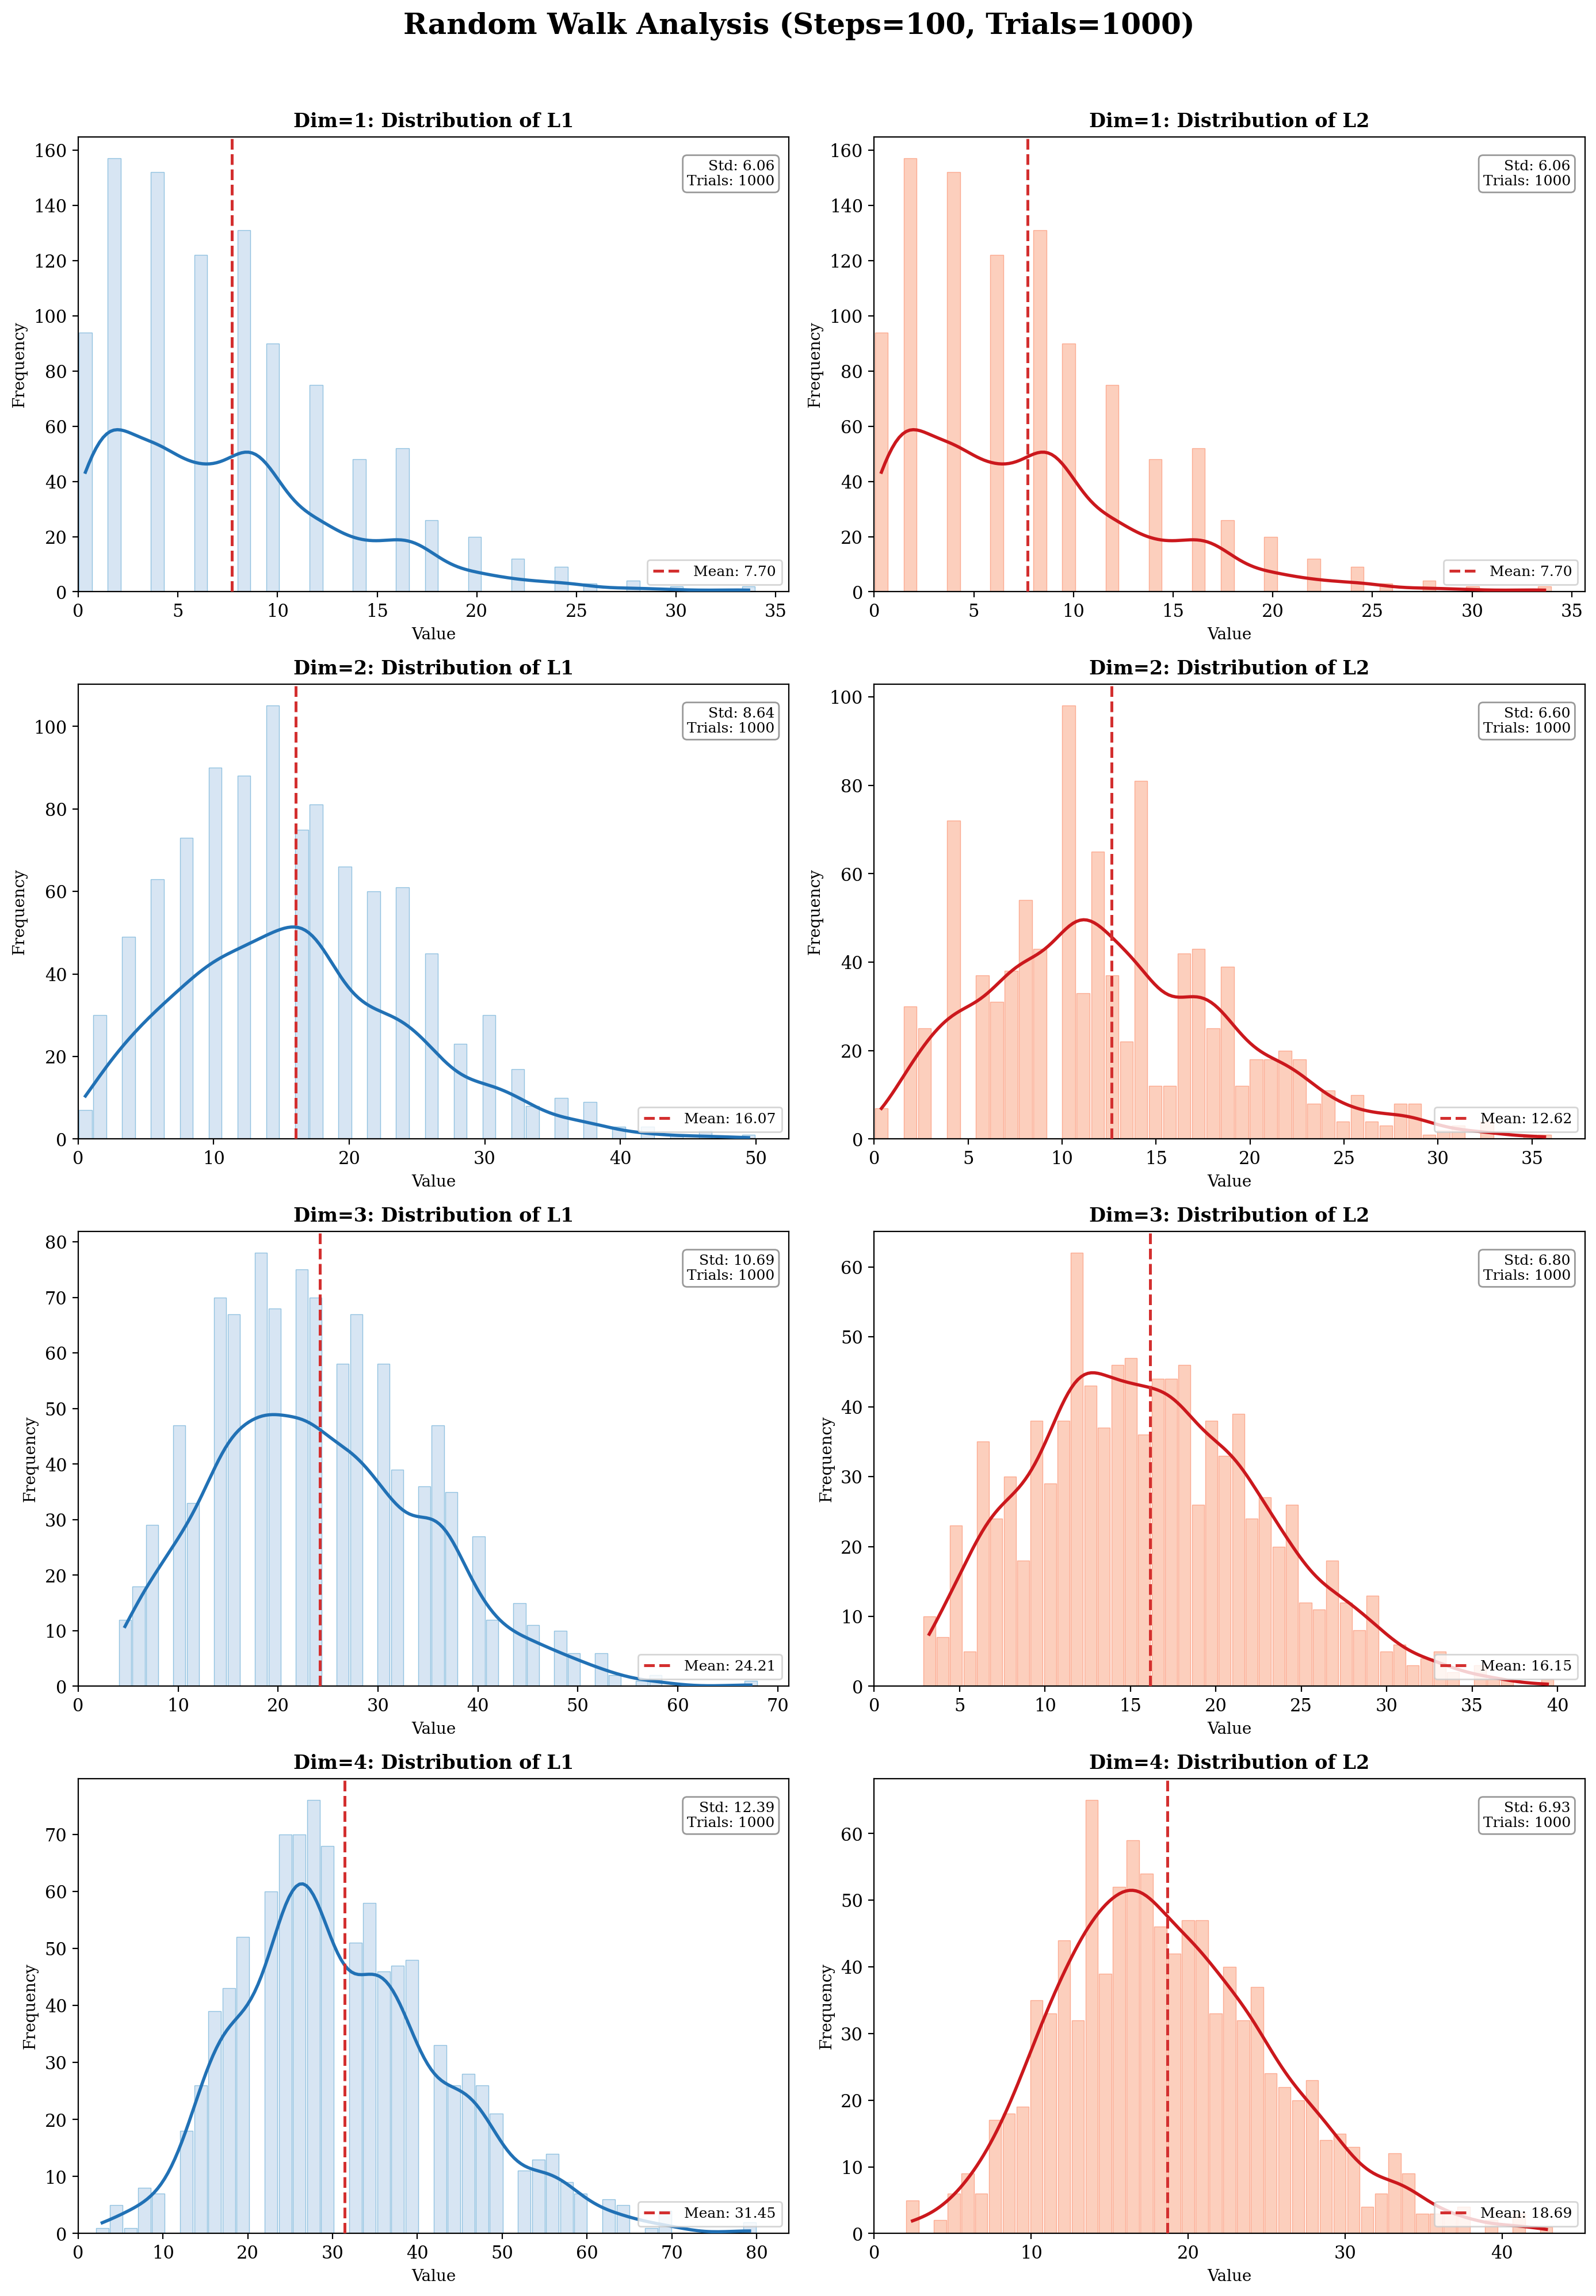
\includegraphics[width=0.95\textwidth]{distance_n100.png}
  \caption{$n=100$ 步模擬結果：各維度的 L1 和 L2 距離分佈}
  \label{fig:dist100}
\end{figure}

\begin{figure}[H]
  \centering
  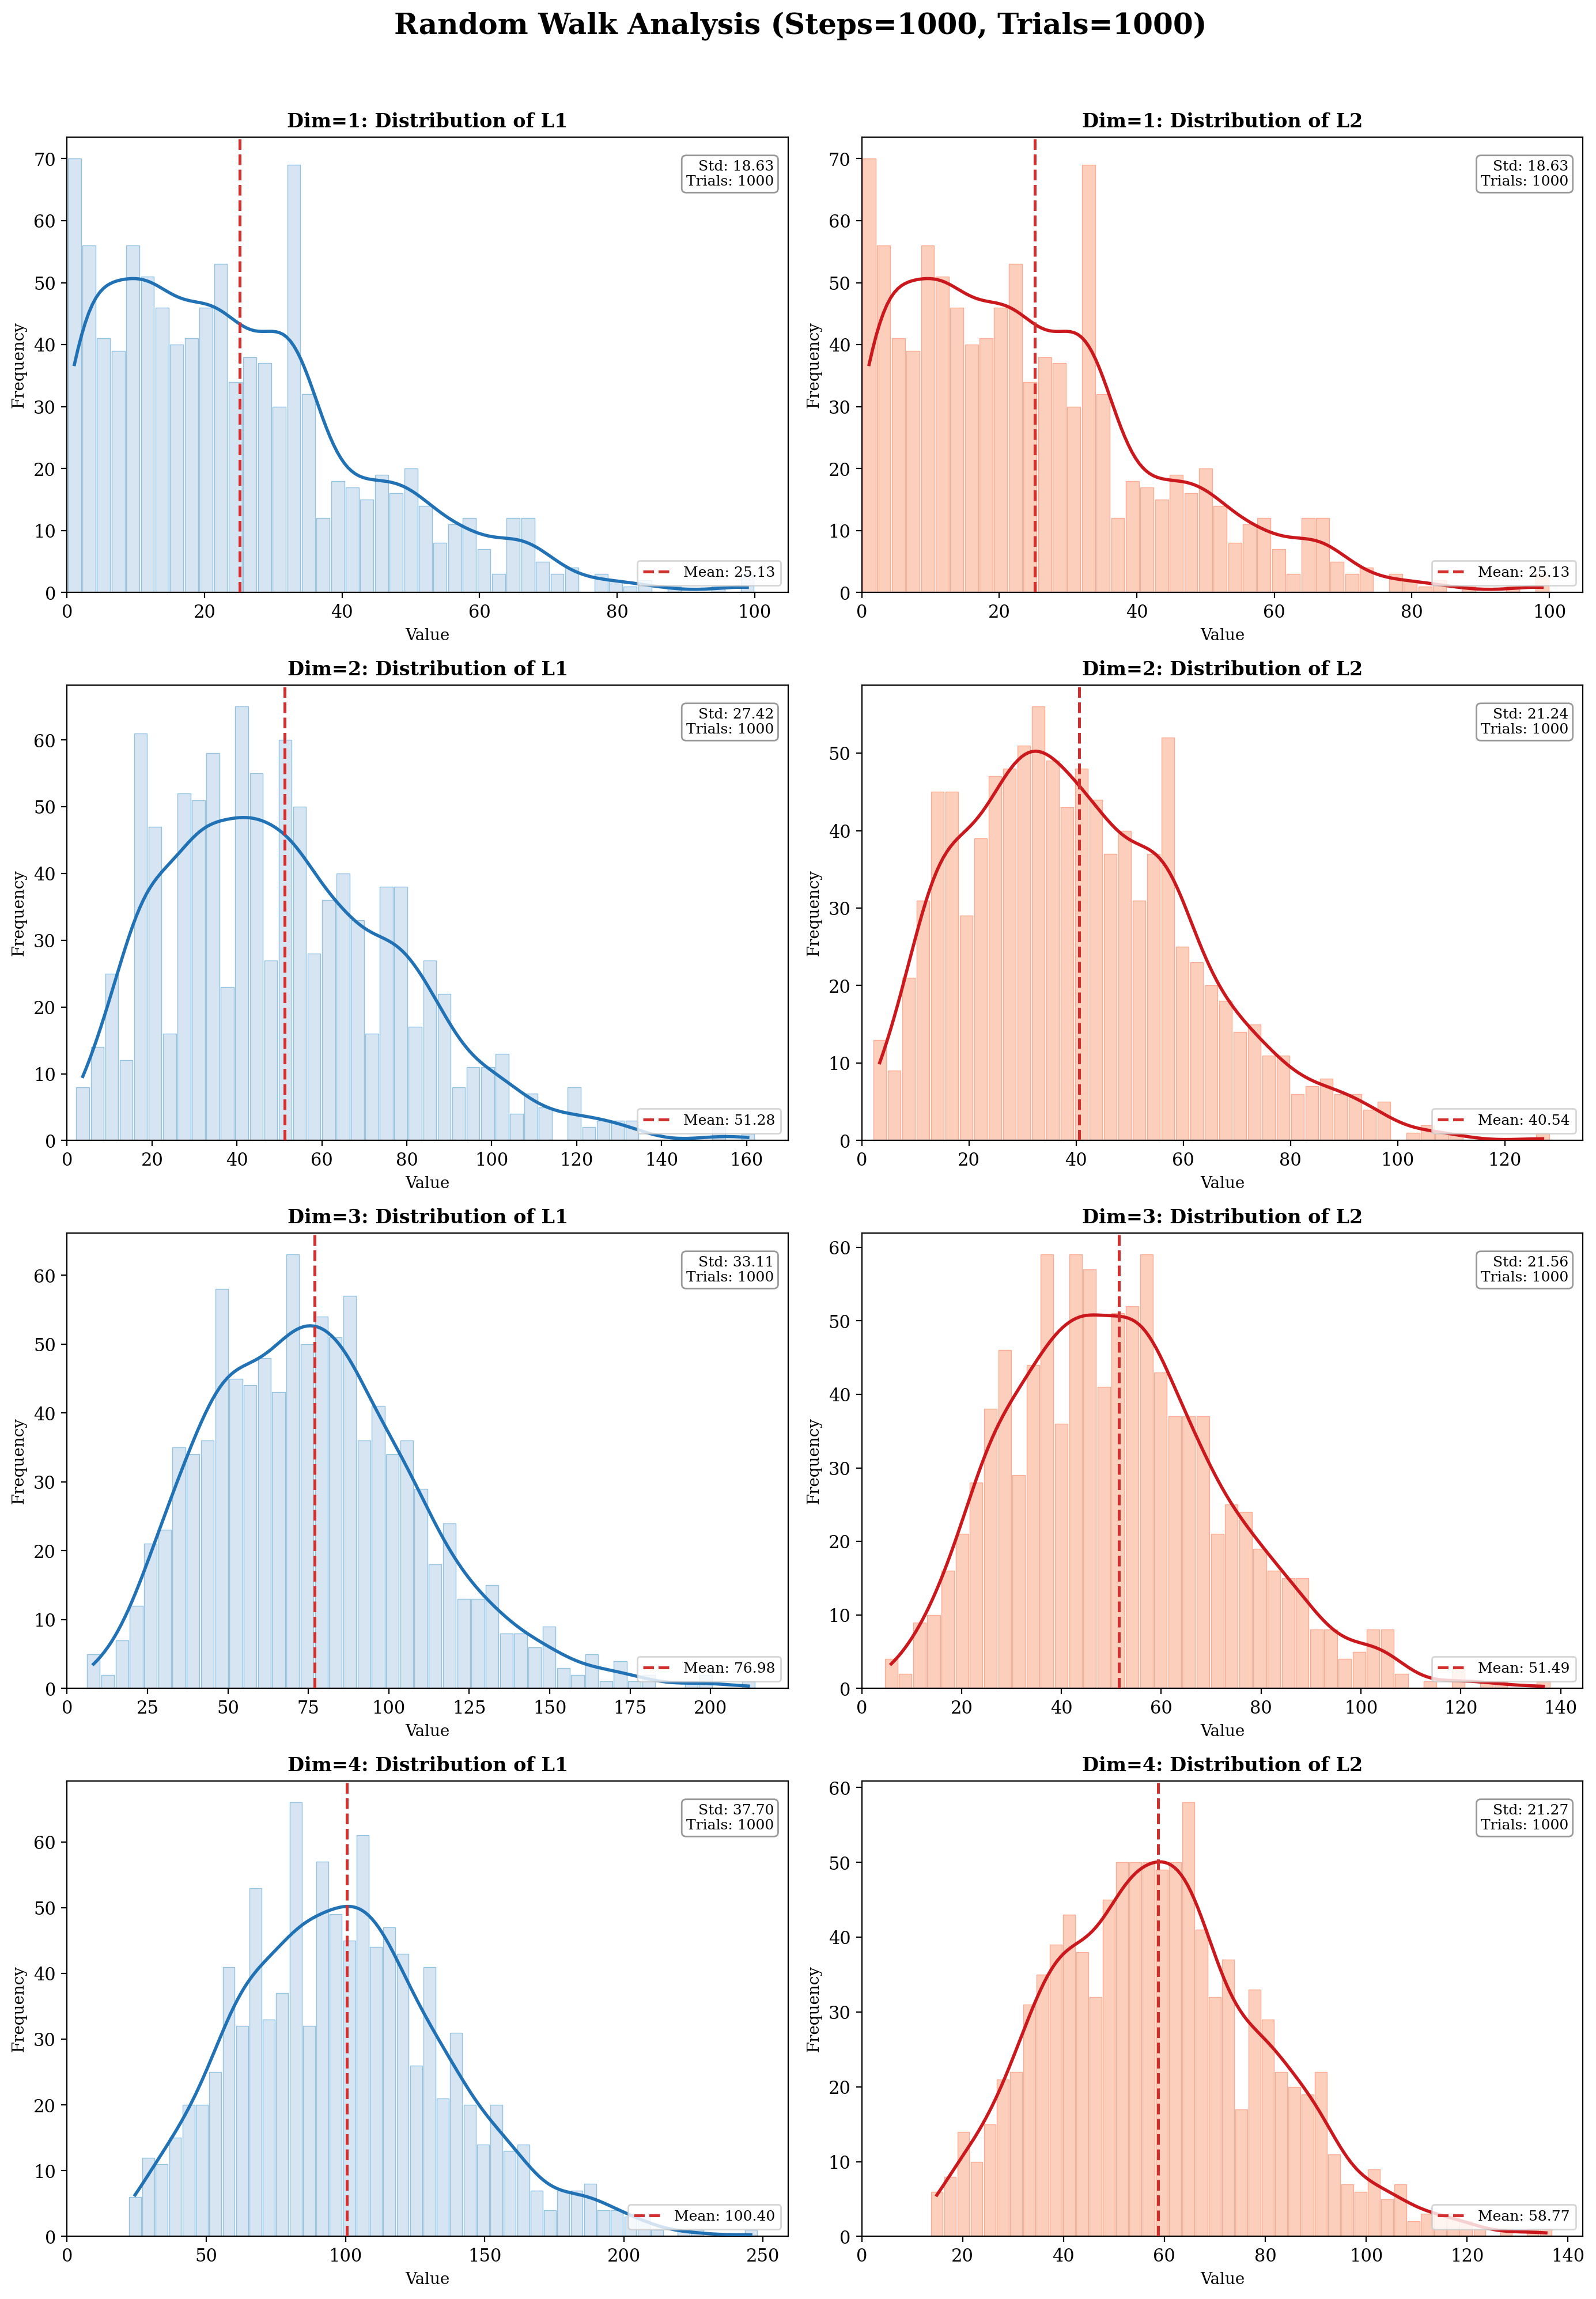
\includegraphics[width=0.95\textwidth]{distance_n1000.png}
  \caption{$n=1000$ 步模擬結果：各維度的 L1 和 L2 距離分佈}
  \label{fig:dist1000}
\end{figure}

\begin{figure}[H]
  \centering
  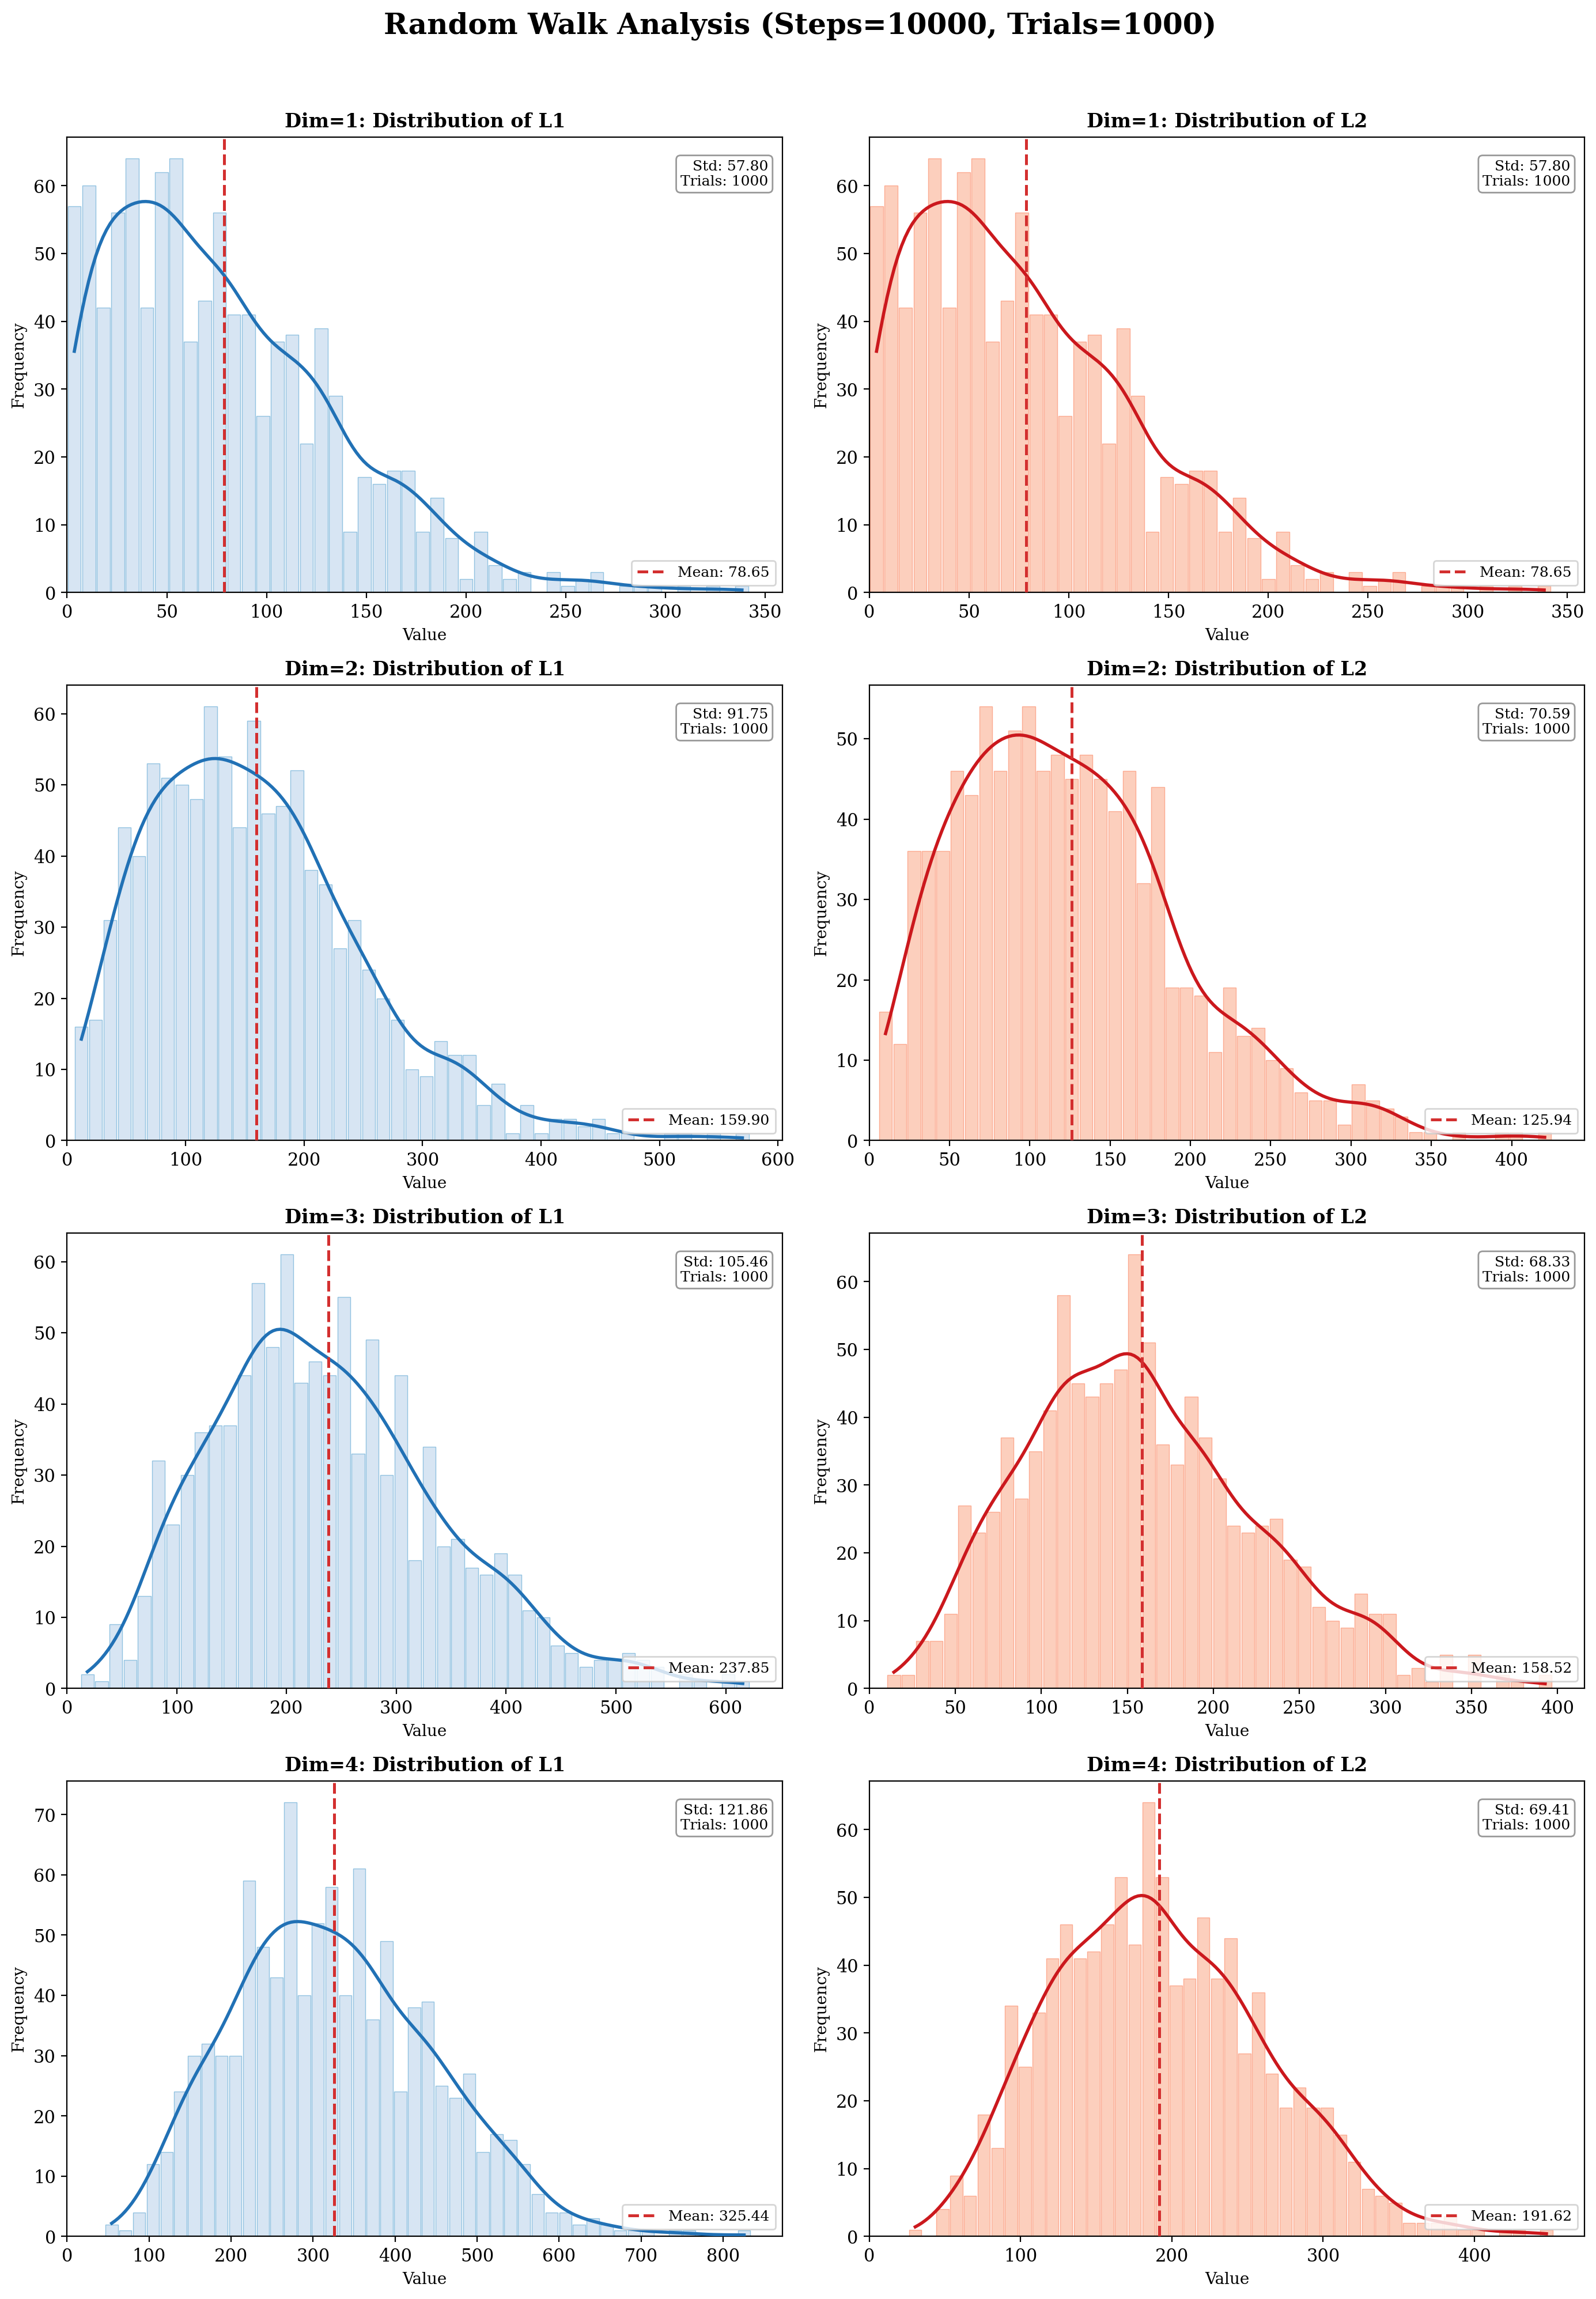
\includegraphics[width=0.95\textwidth]{distance_n10000.png}
  \caption{$n=10000$ 步模擬結果：各維度的 L1 和 L2 距離分佈}
  \label{fig:dist10000}
\end{figure}

\begin{figure}[H]
  \centering
  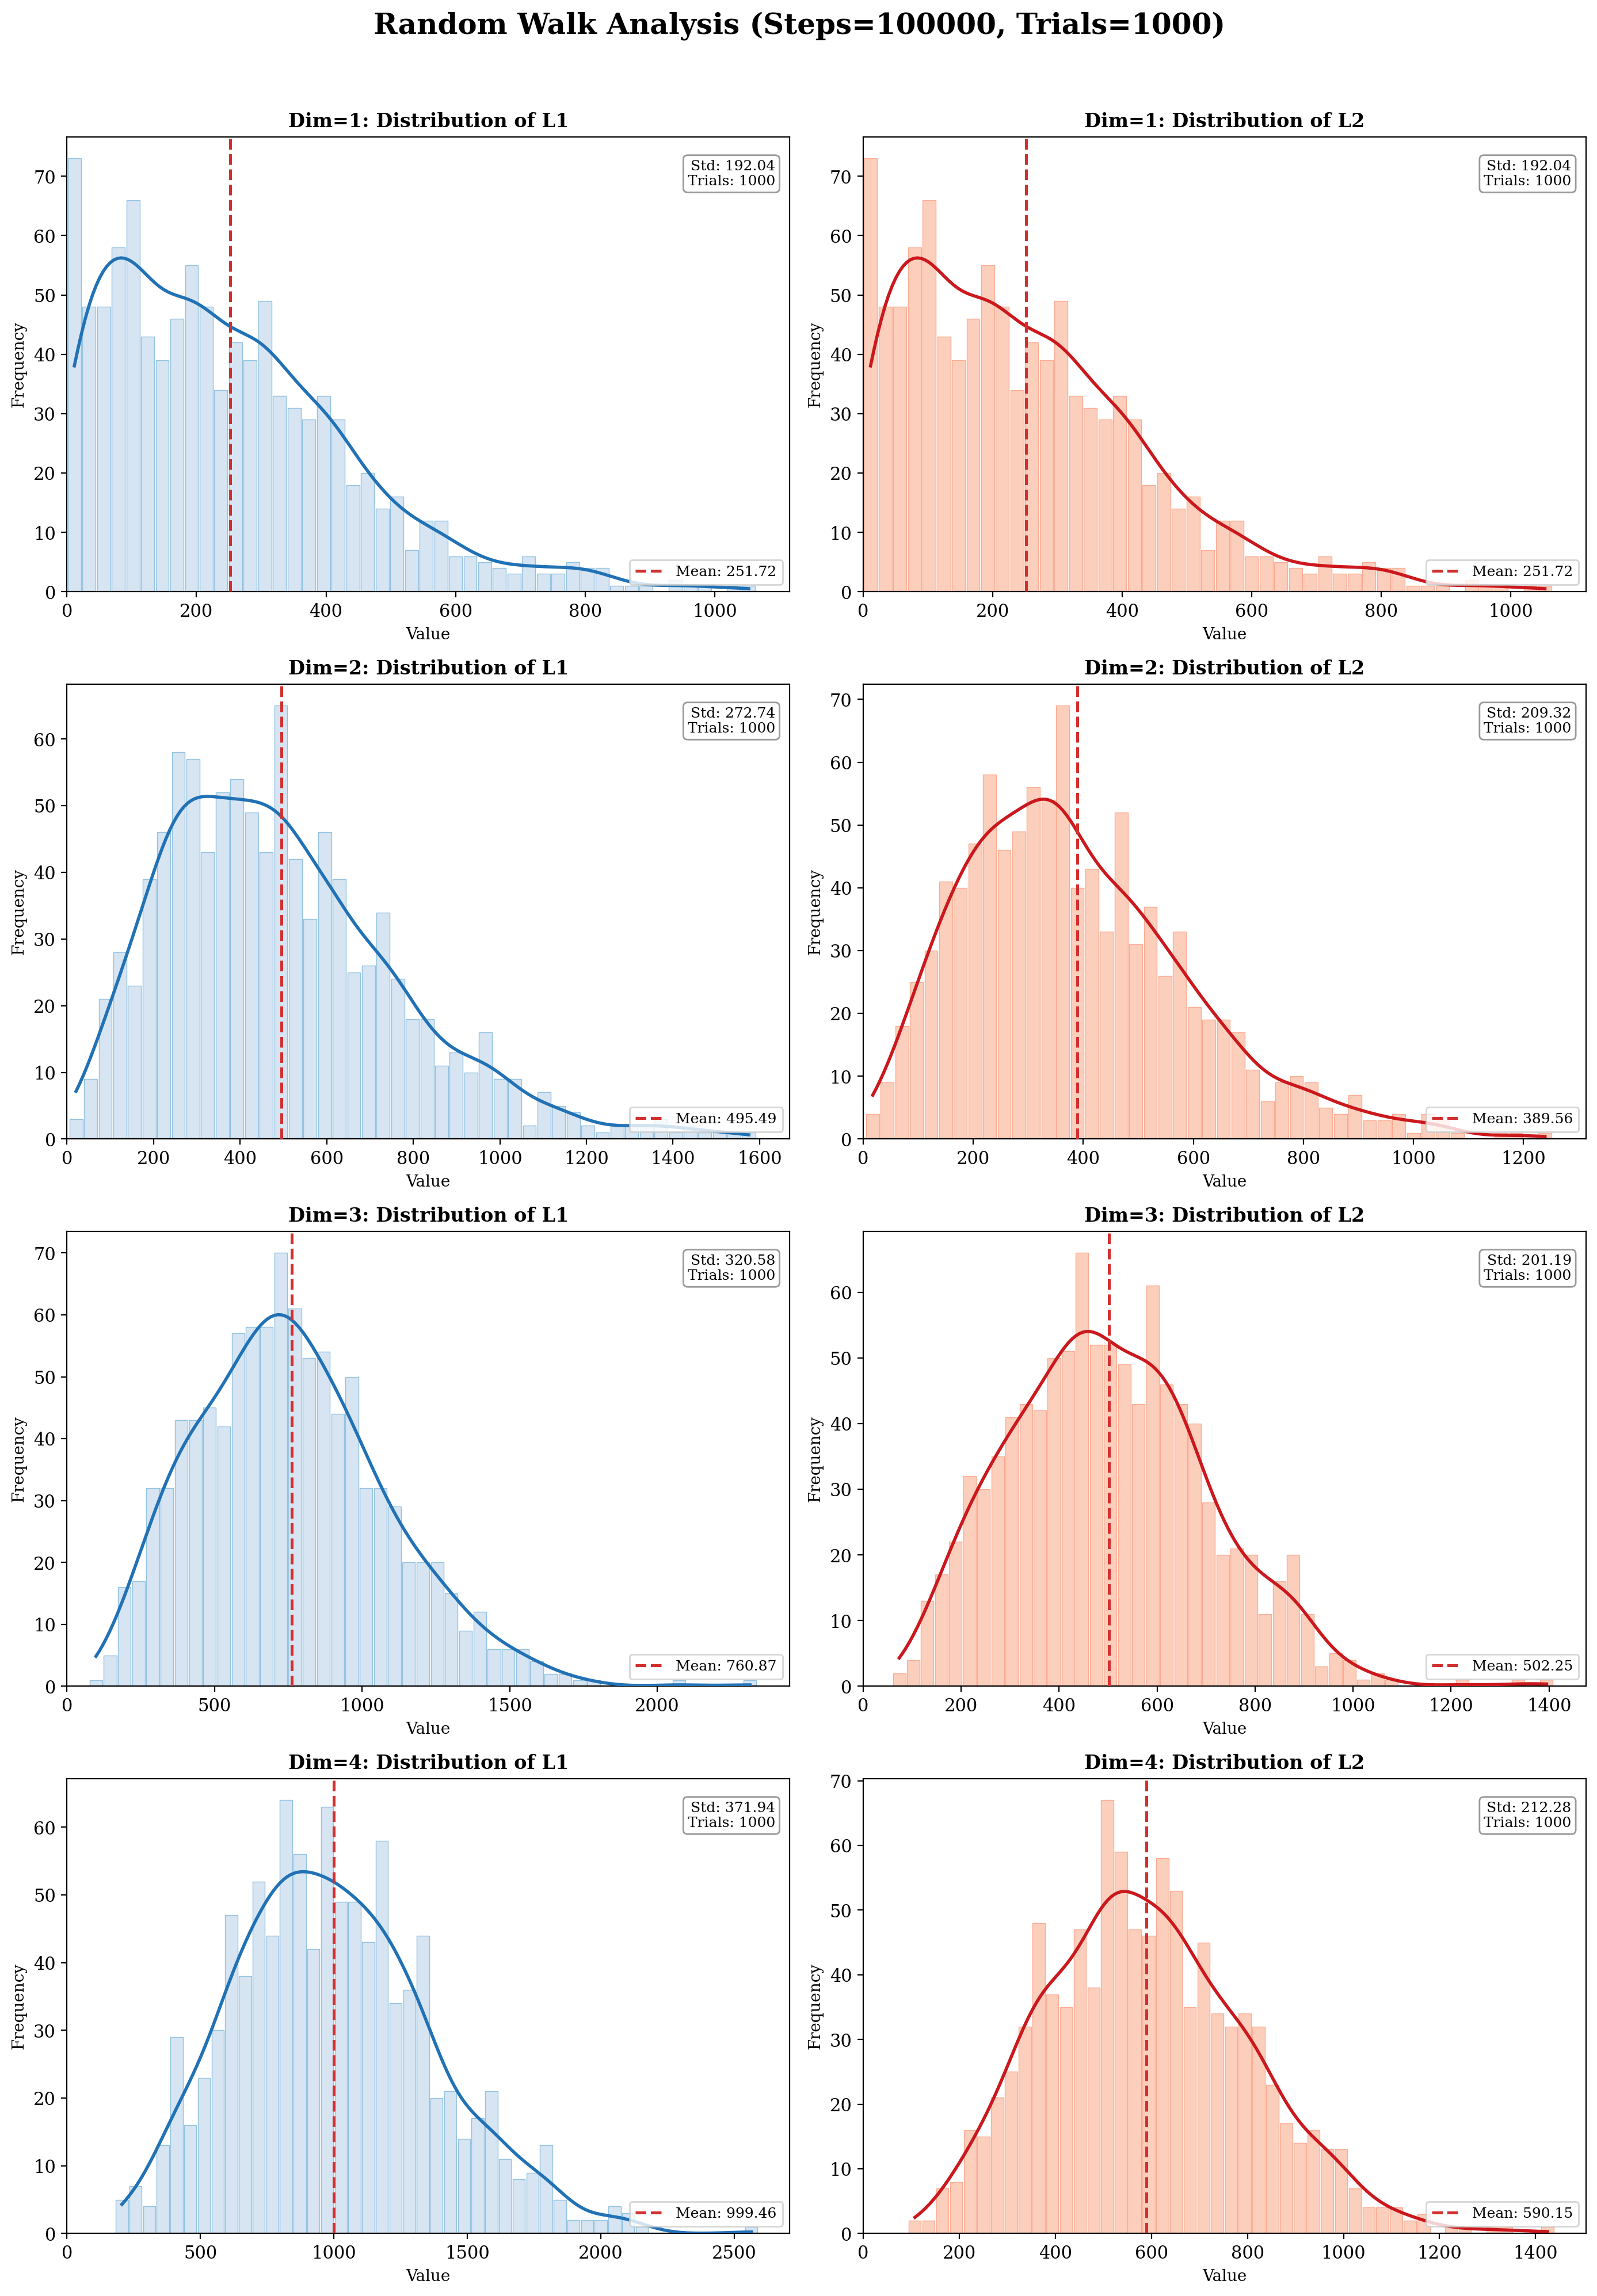
\includegraphics[width=0.95\textwidth]{distance_n100000.png}
  \caption{$n=100000$ 步模擬結果：各維度的 L1 和 L2 距離分佈}
  \label{fig:dist100000}
\end{figure}

\begin{figure}[H]
  \centering
  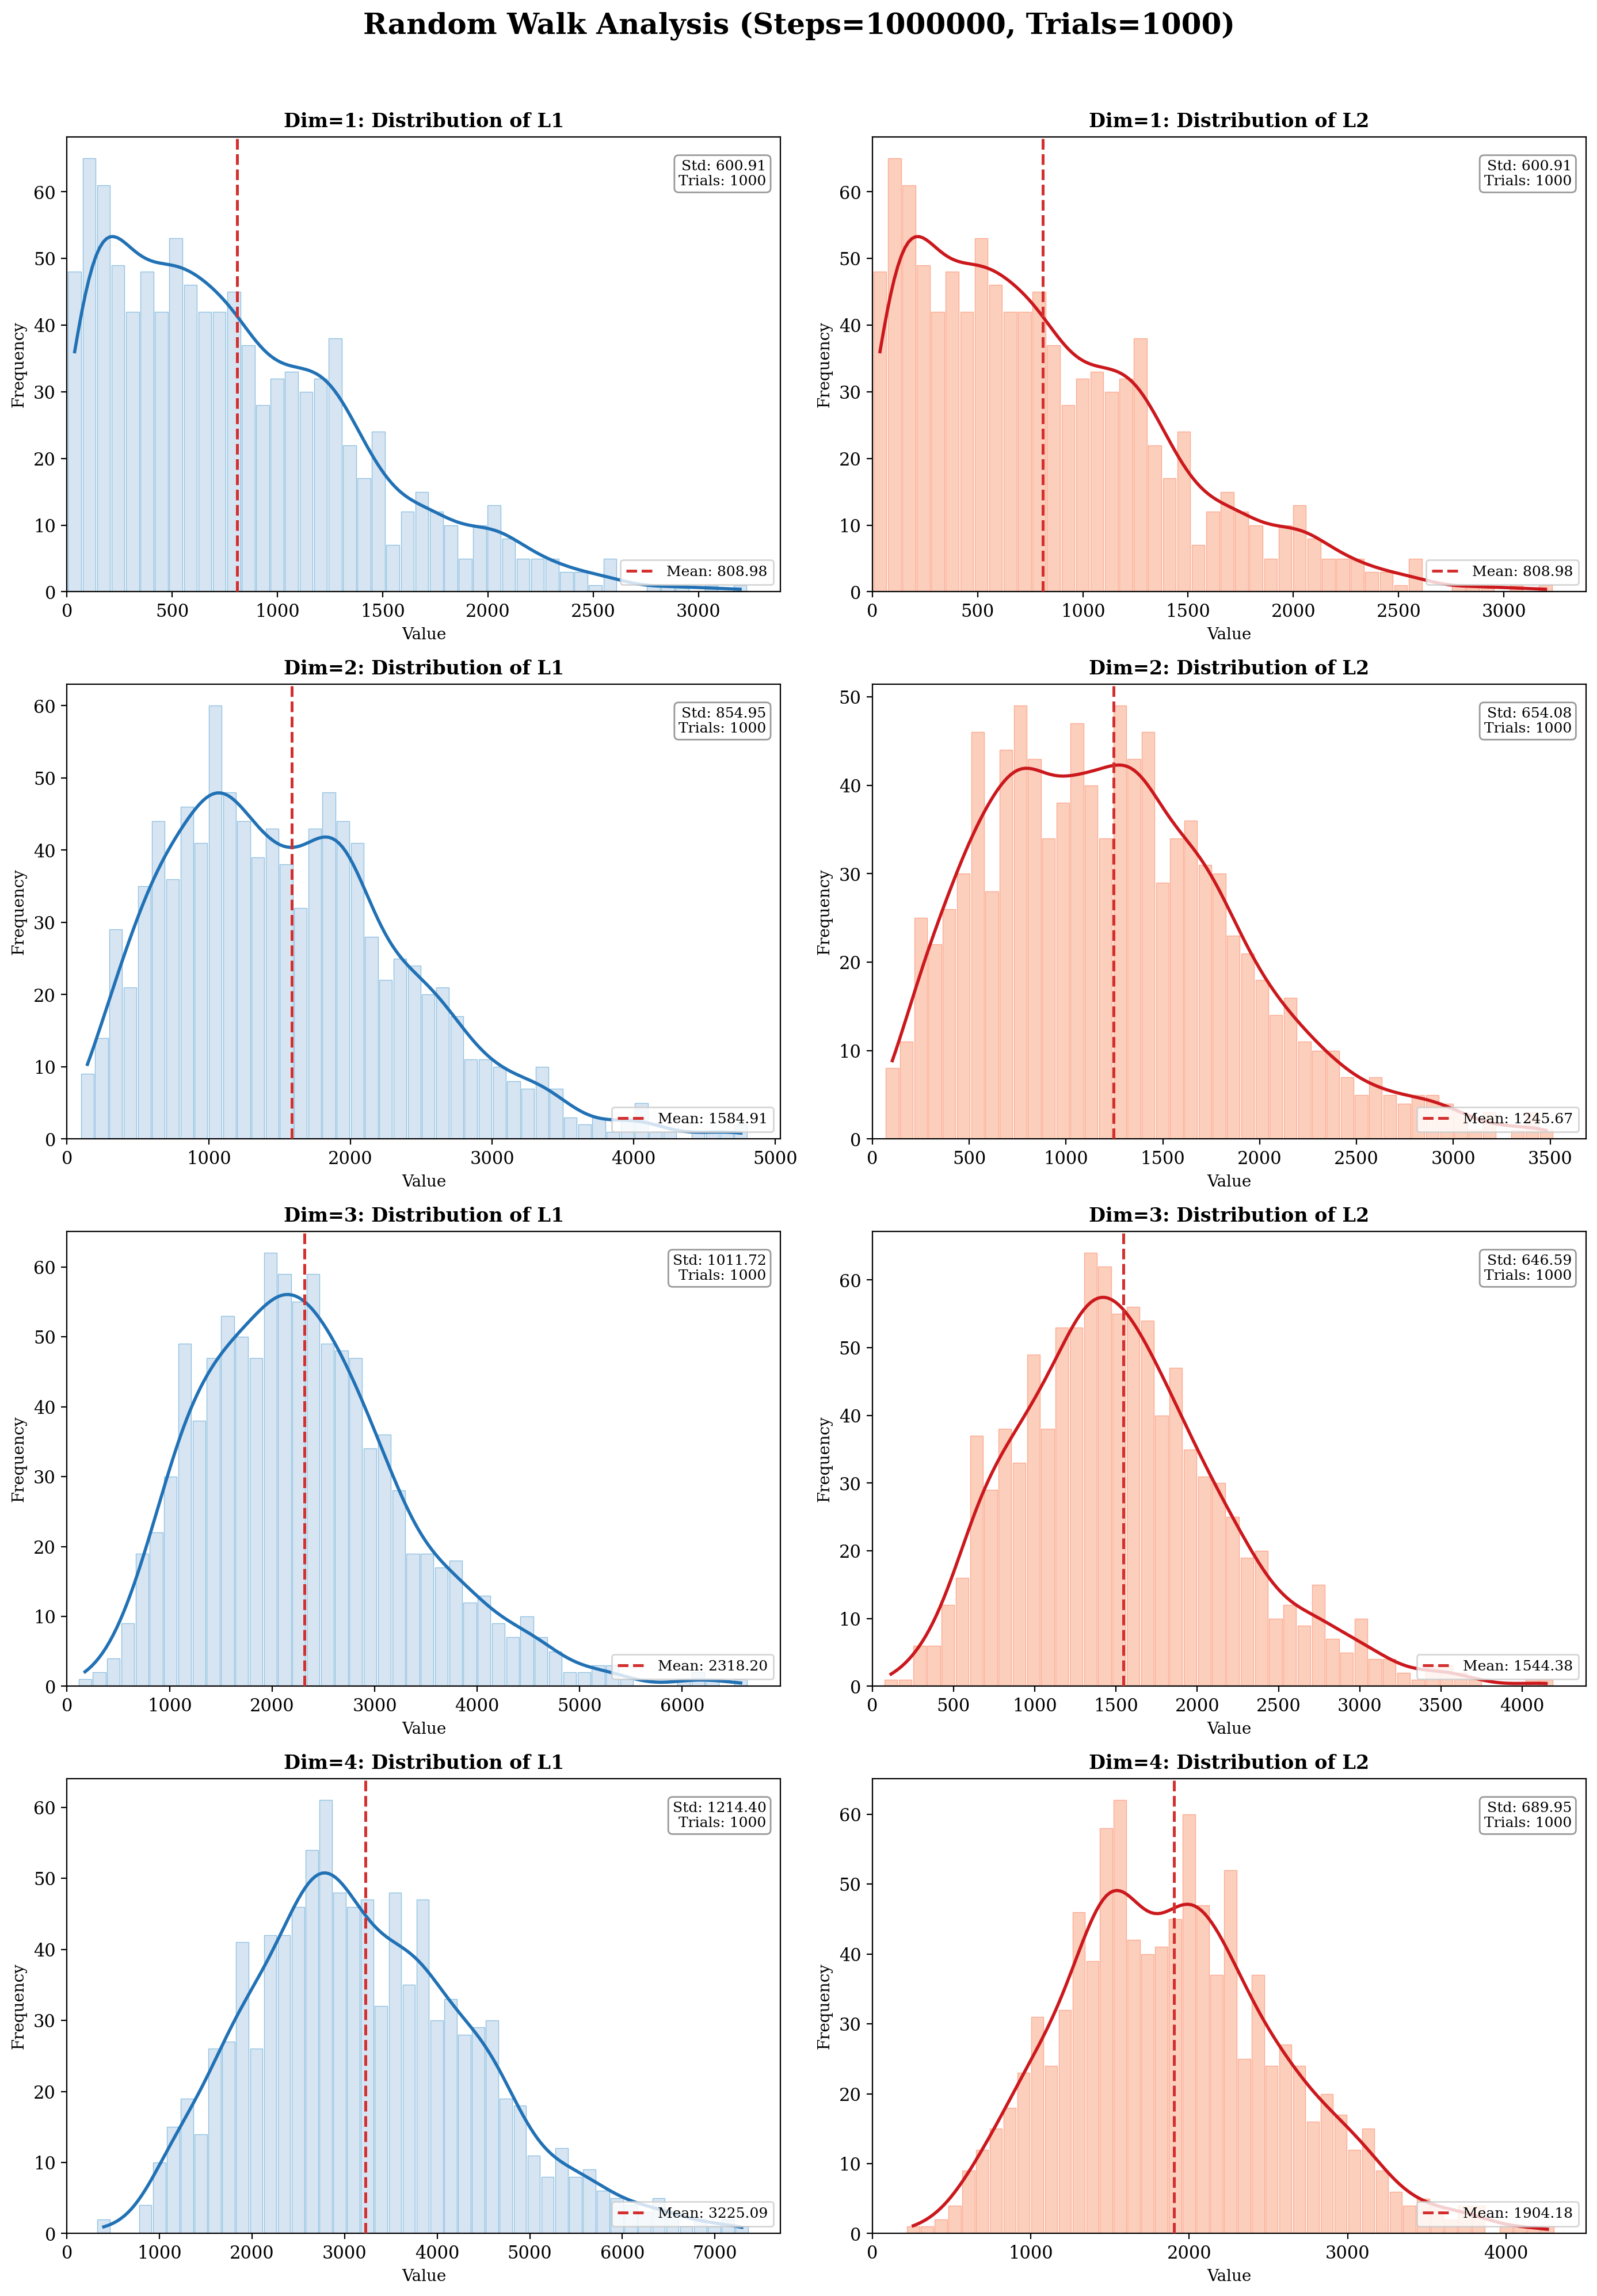
\includegraphics[width=0.95\textwidth]{distance_n1000000.png}
  \caption{$n=1000000$ 步模擬結果：各維度的 L1 和 L2 距離分佈}
  \label{fig:dist1000000}
\end{figure}

從圖中可以觀察到：
\begin{itemize}[nosep]
  \item 隨著 $n$ 增大，距離分佈逐漸展寬，且 peak 向右移動
  \item 分佈形狀近似 half-normal 或 Rayleigh 分佈，符合 random walk 理論的預期
  \item 在固定 $n$ 下，維度越高，L2 距離的期望值也越大（因為各維度的 variance 會累加）
\end{itemize}

\subsection{距離 Scaling 分析}

圖~\ref{fig:scaling} 展示平均距離與 $\sqrt{n}$ 的 scaling 關係。

\begin{figure}[H]
  \centering
  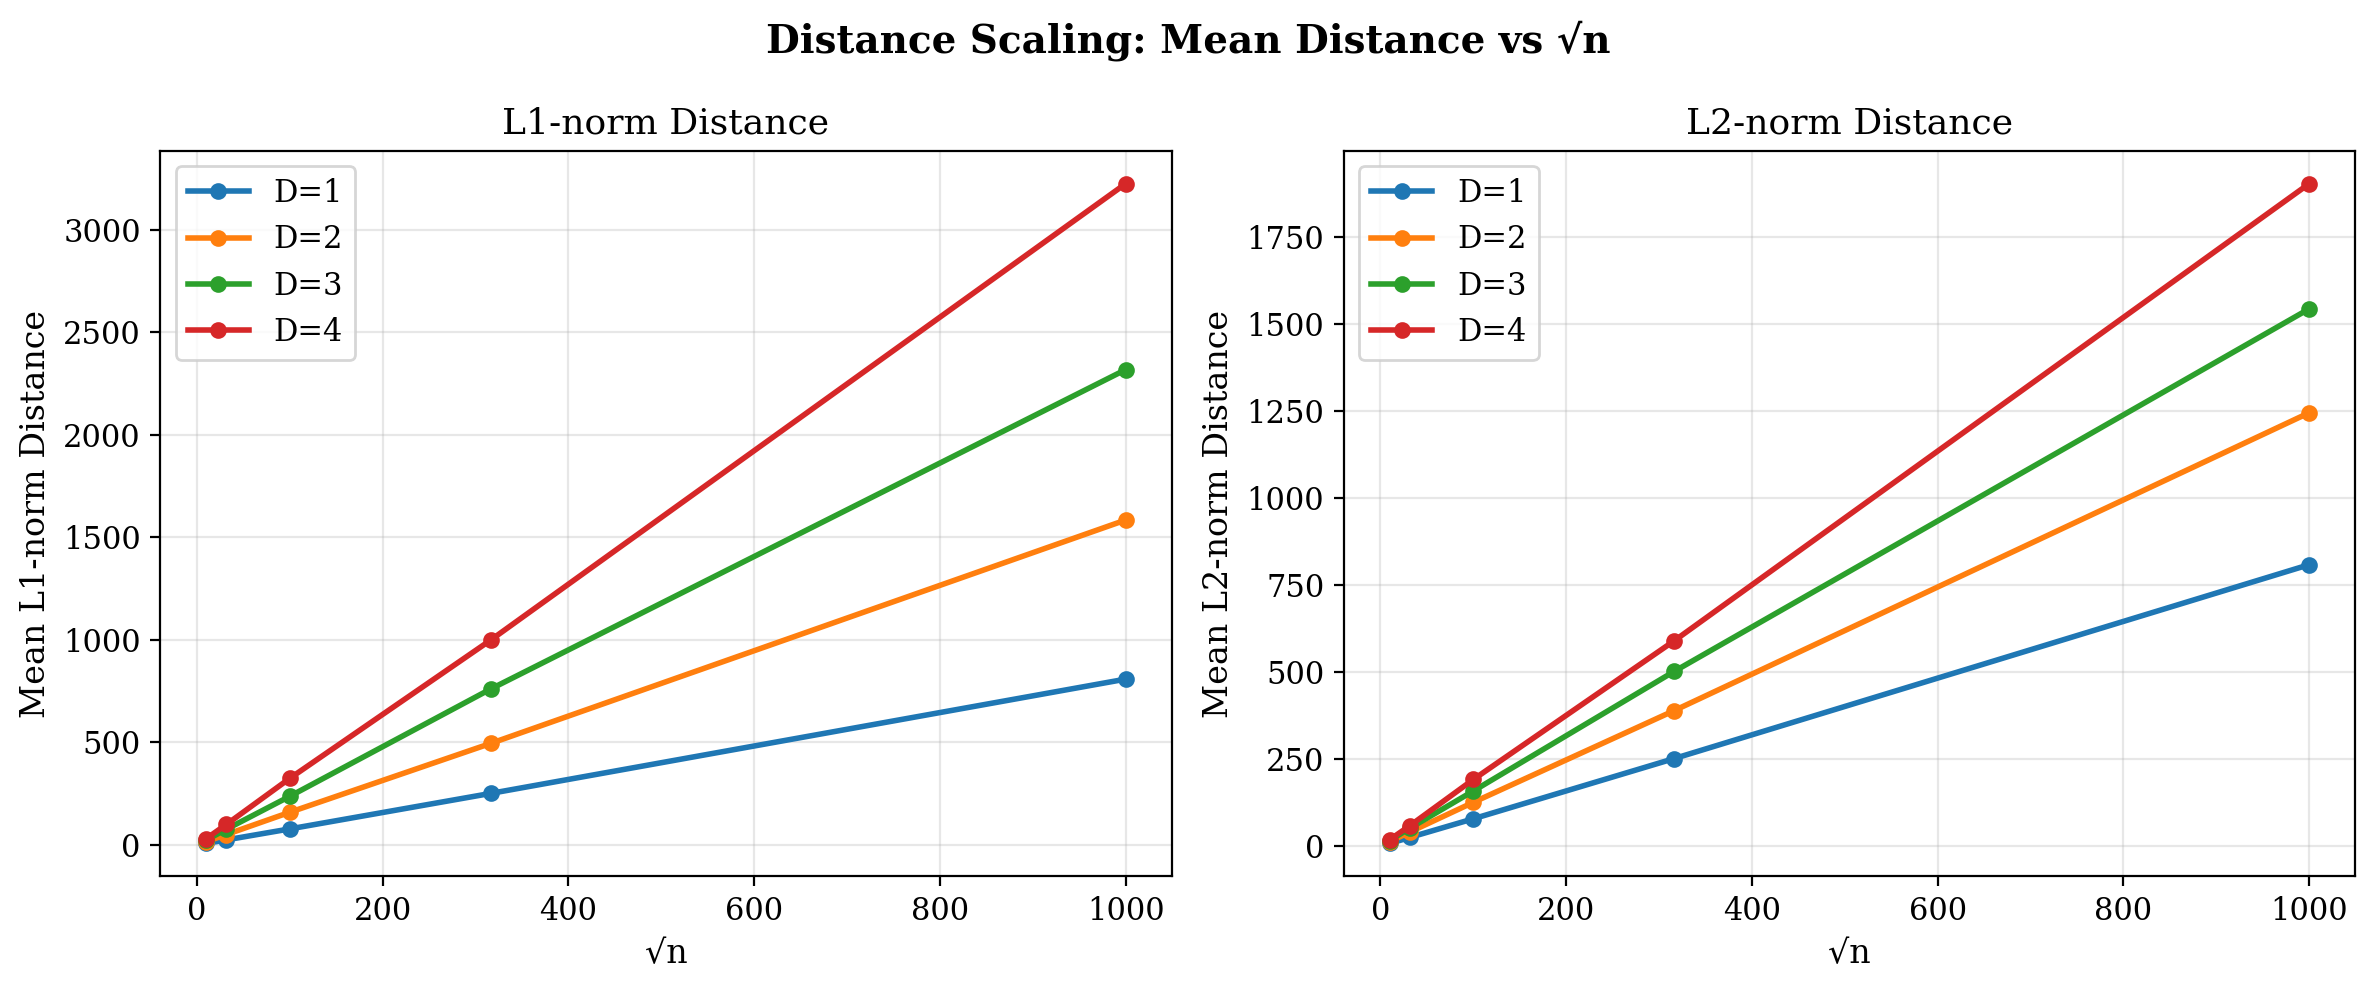
\includegraphics[width=0.85\textwidth]{distance_scaling.png}
  \caption{平均 L1 和 L2 距離 vs $\sqrt{n}$}
  \label{fig:scaling}
\end{figure}

由圖可見，平均距離與 $\sqrt{n}$ 呈線性關係，
驗證了 random walk 的基本理論結果：
\begin{equation}
  \mathbb{E}[\|\mathbf{x}^{(n)}\|_2] \propto \sqrt{n}
\end{equation}

\subsection{象限（Section）停留比例}

圖~\ref{fig:sec1}--\ref{fig:sec4} 展示各維度下、各 section 的平均停留比例。
在 $D$ 維空間中有 $2^D$ 個 section。

\begin{figure}[H]
  \centering
  \begin{subfigure}[b]{0.48\textwidth}
    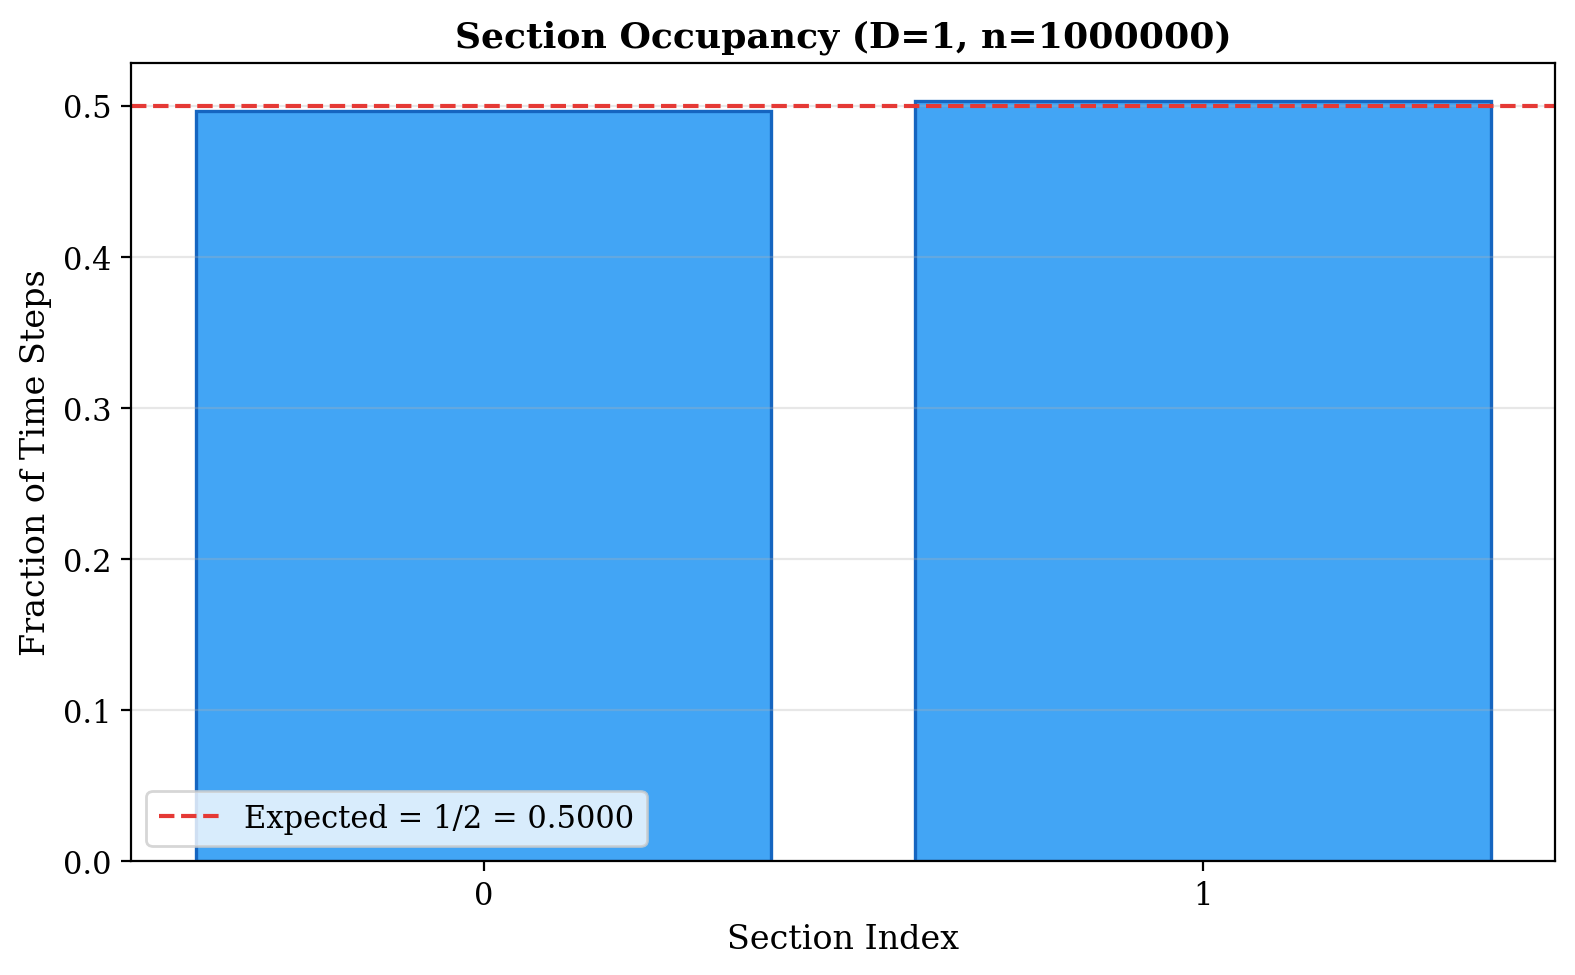
\includegraphics[width=\textwidth]{section_D1.png}
    \caption{$D=1$（2 sections）}
    \label{fig:sec1}
  \end{subfigure}
  \hfill
  \begin{subfigure}[b]{0.48\textwidth}
    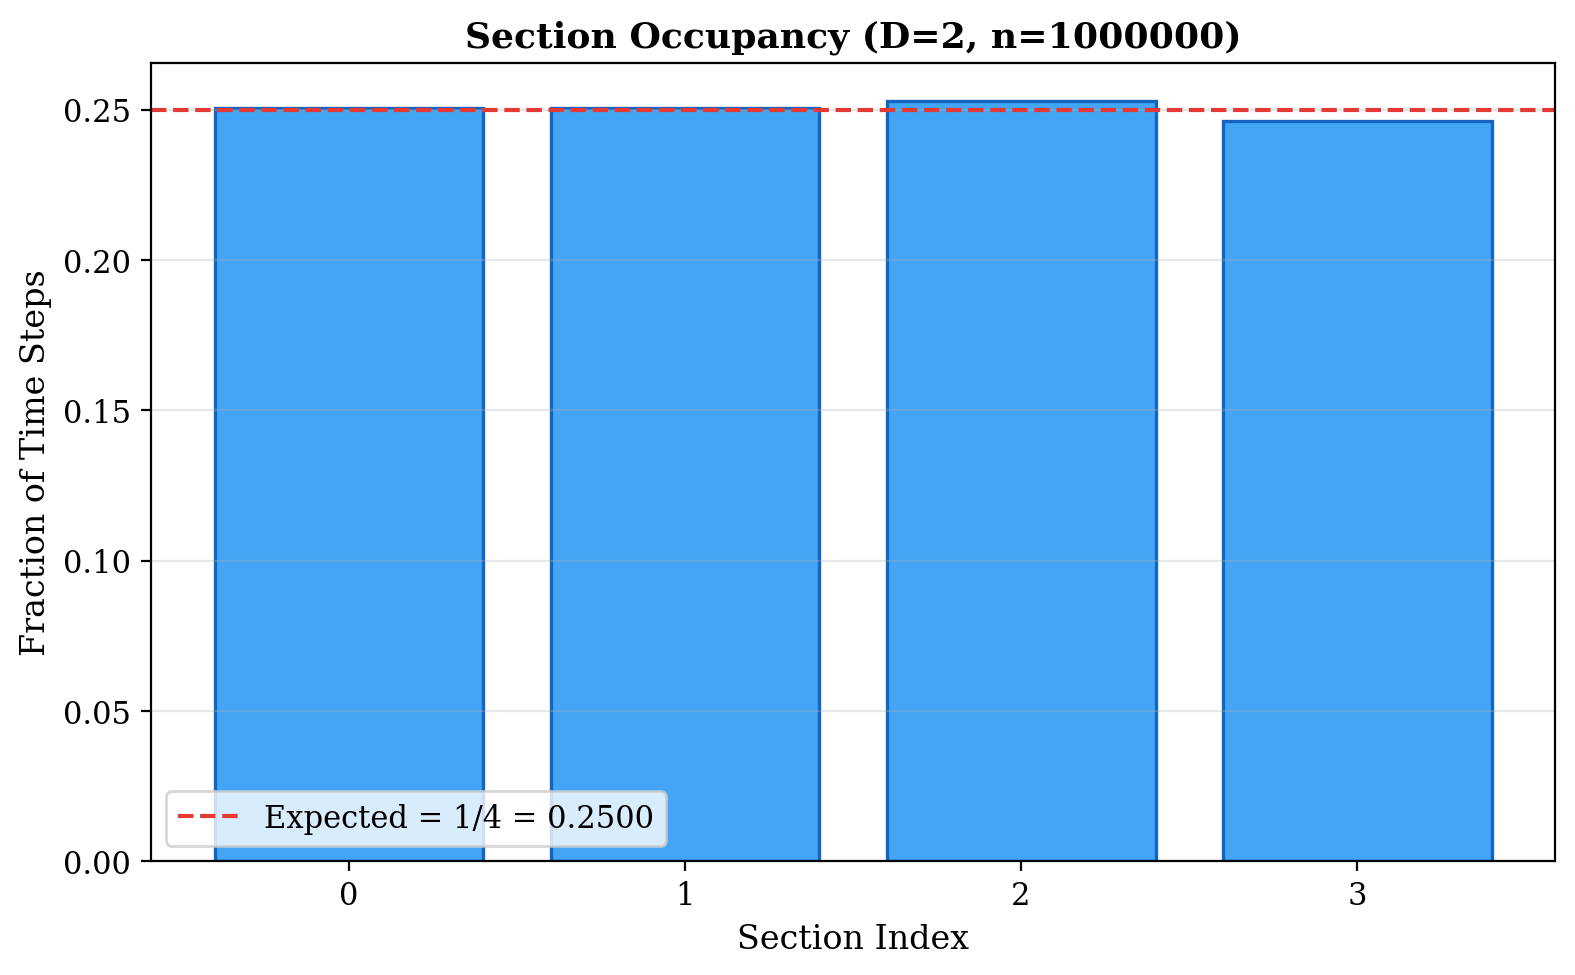
\includegraphics[width=\textwidth]{section_D2.png}
    \caption{$D=2$（4 quadrants）}
    \label{fig:sec2}
  \end{subfigure}
  \\[1em]
  \begin{subfigure}[b]{0.48\textwidth}
    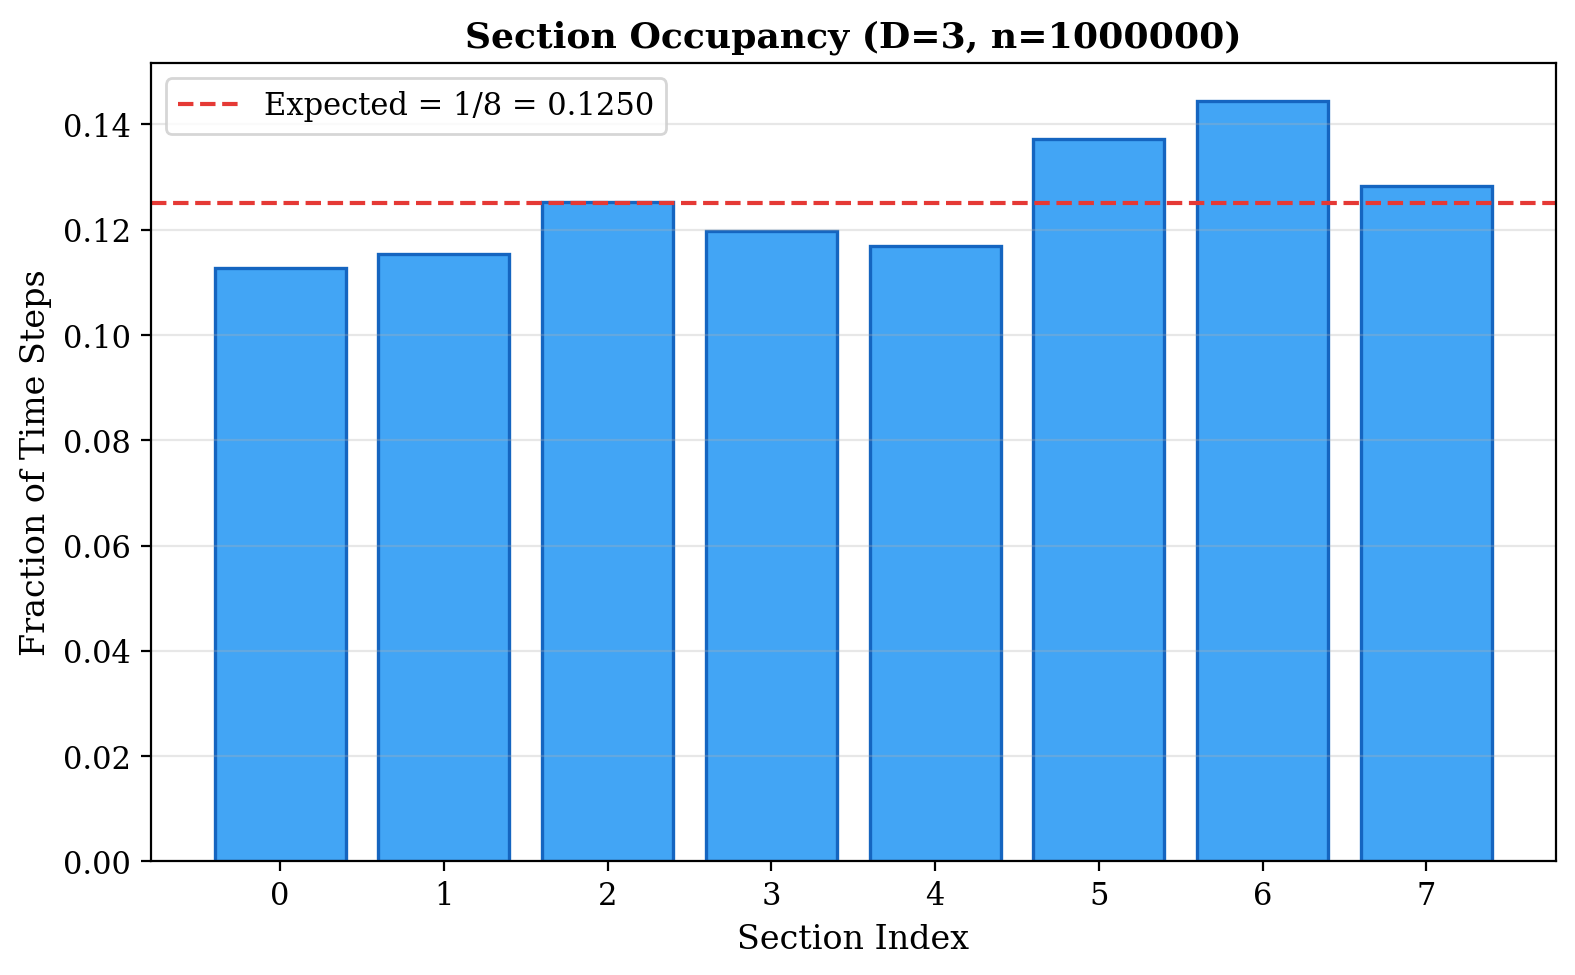
\includegraphics[width=\textwidth]{section_D3.png}
    \caption{$D=3$（8 octants）}
    \label{fig:sec3}
  \end{subfigure}
  \hfill
  \begin{subfigure}[b]{0.48\textwidth}
    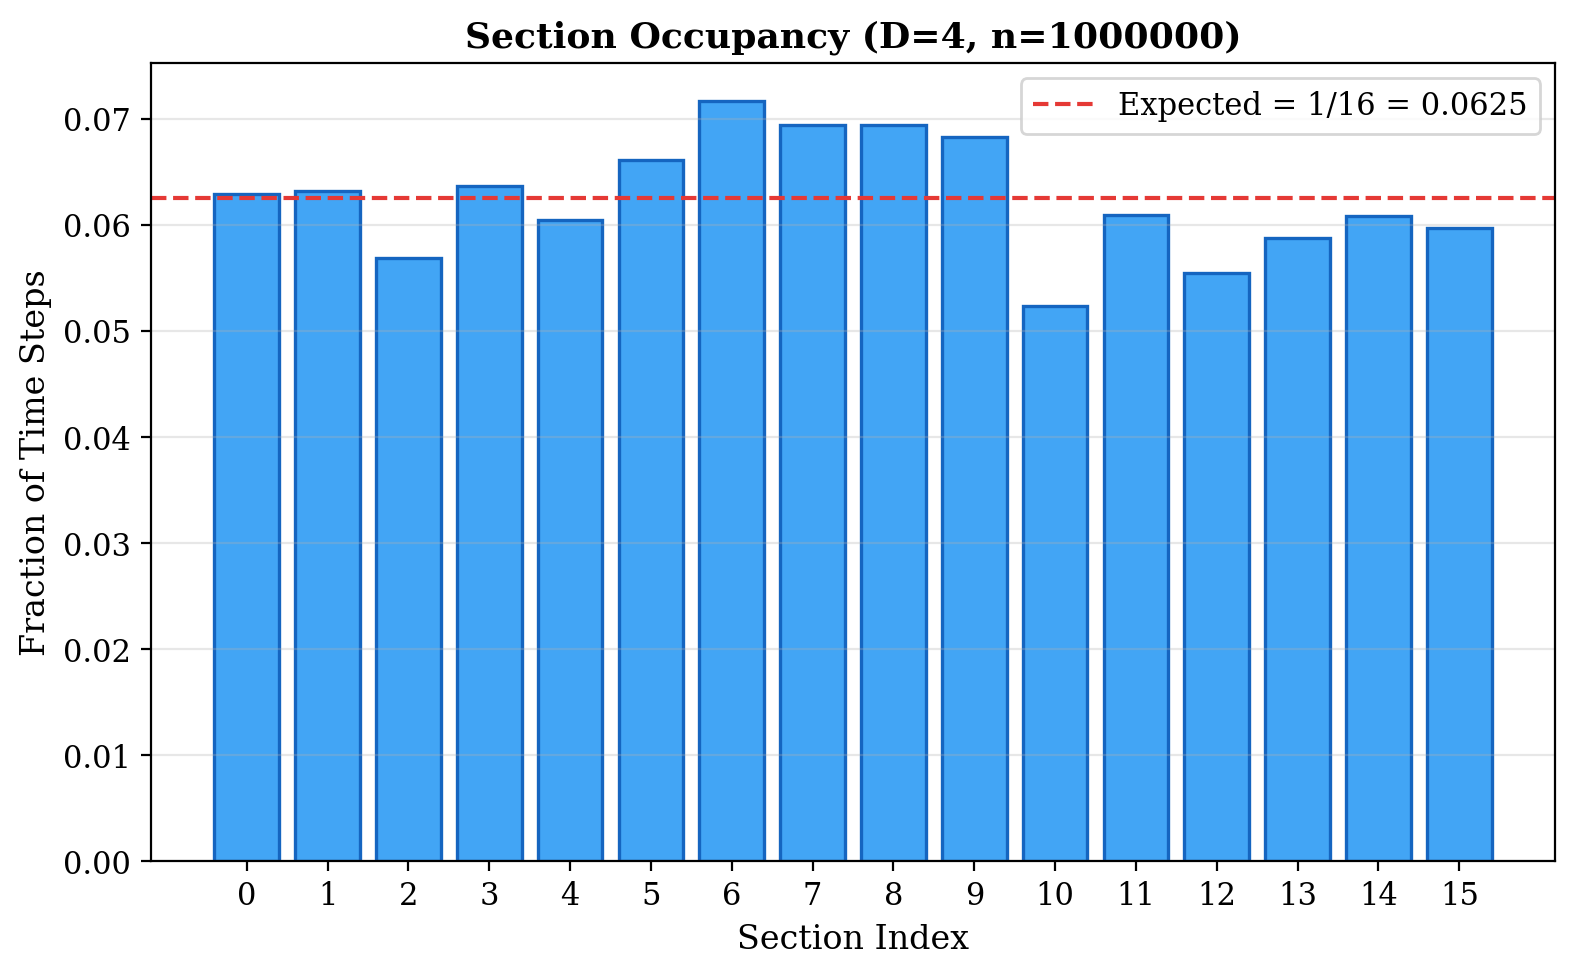
\includegraphics[width=\textwidth]{section_D4.png}
    \caption{$D=4$（16 sections）}
    \label{fig:sec4}
  \end{subfigure}
  \caption{各維度的 section 停留比例。紅色虛線為理論期望值 $1/2^D$。}
  \label{fig:sections}
\end{figure}

結果顯示各 section 的停留比例非常接近均勻分佈（$1/2^D$），
這是因為 random walk 在各維度上是獨立且對稱的，
驗證了模擬的正確性。

\subsection{回到原點分析}

\subsubsection{首次回到原點的分佈}

圖~\ref{fig:return} 展示各維度下首次回到原點的 step 數分佈。

\begin{figure}[H]
  \centering
  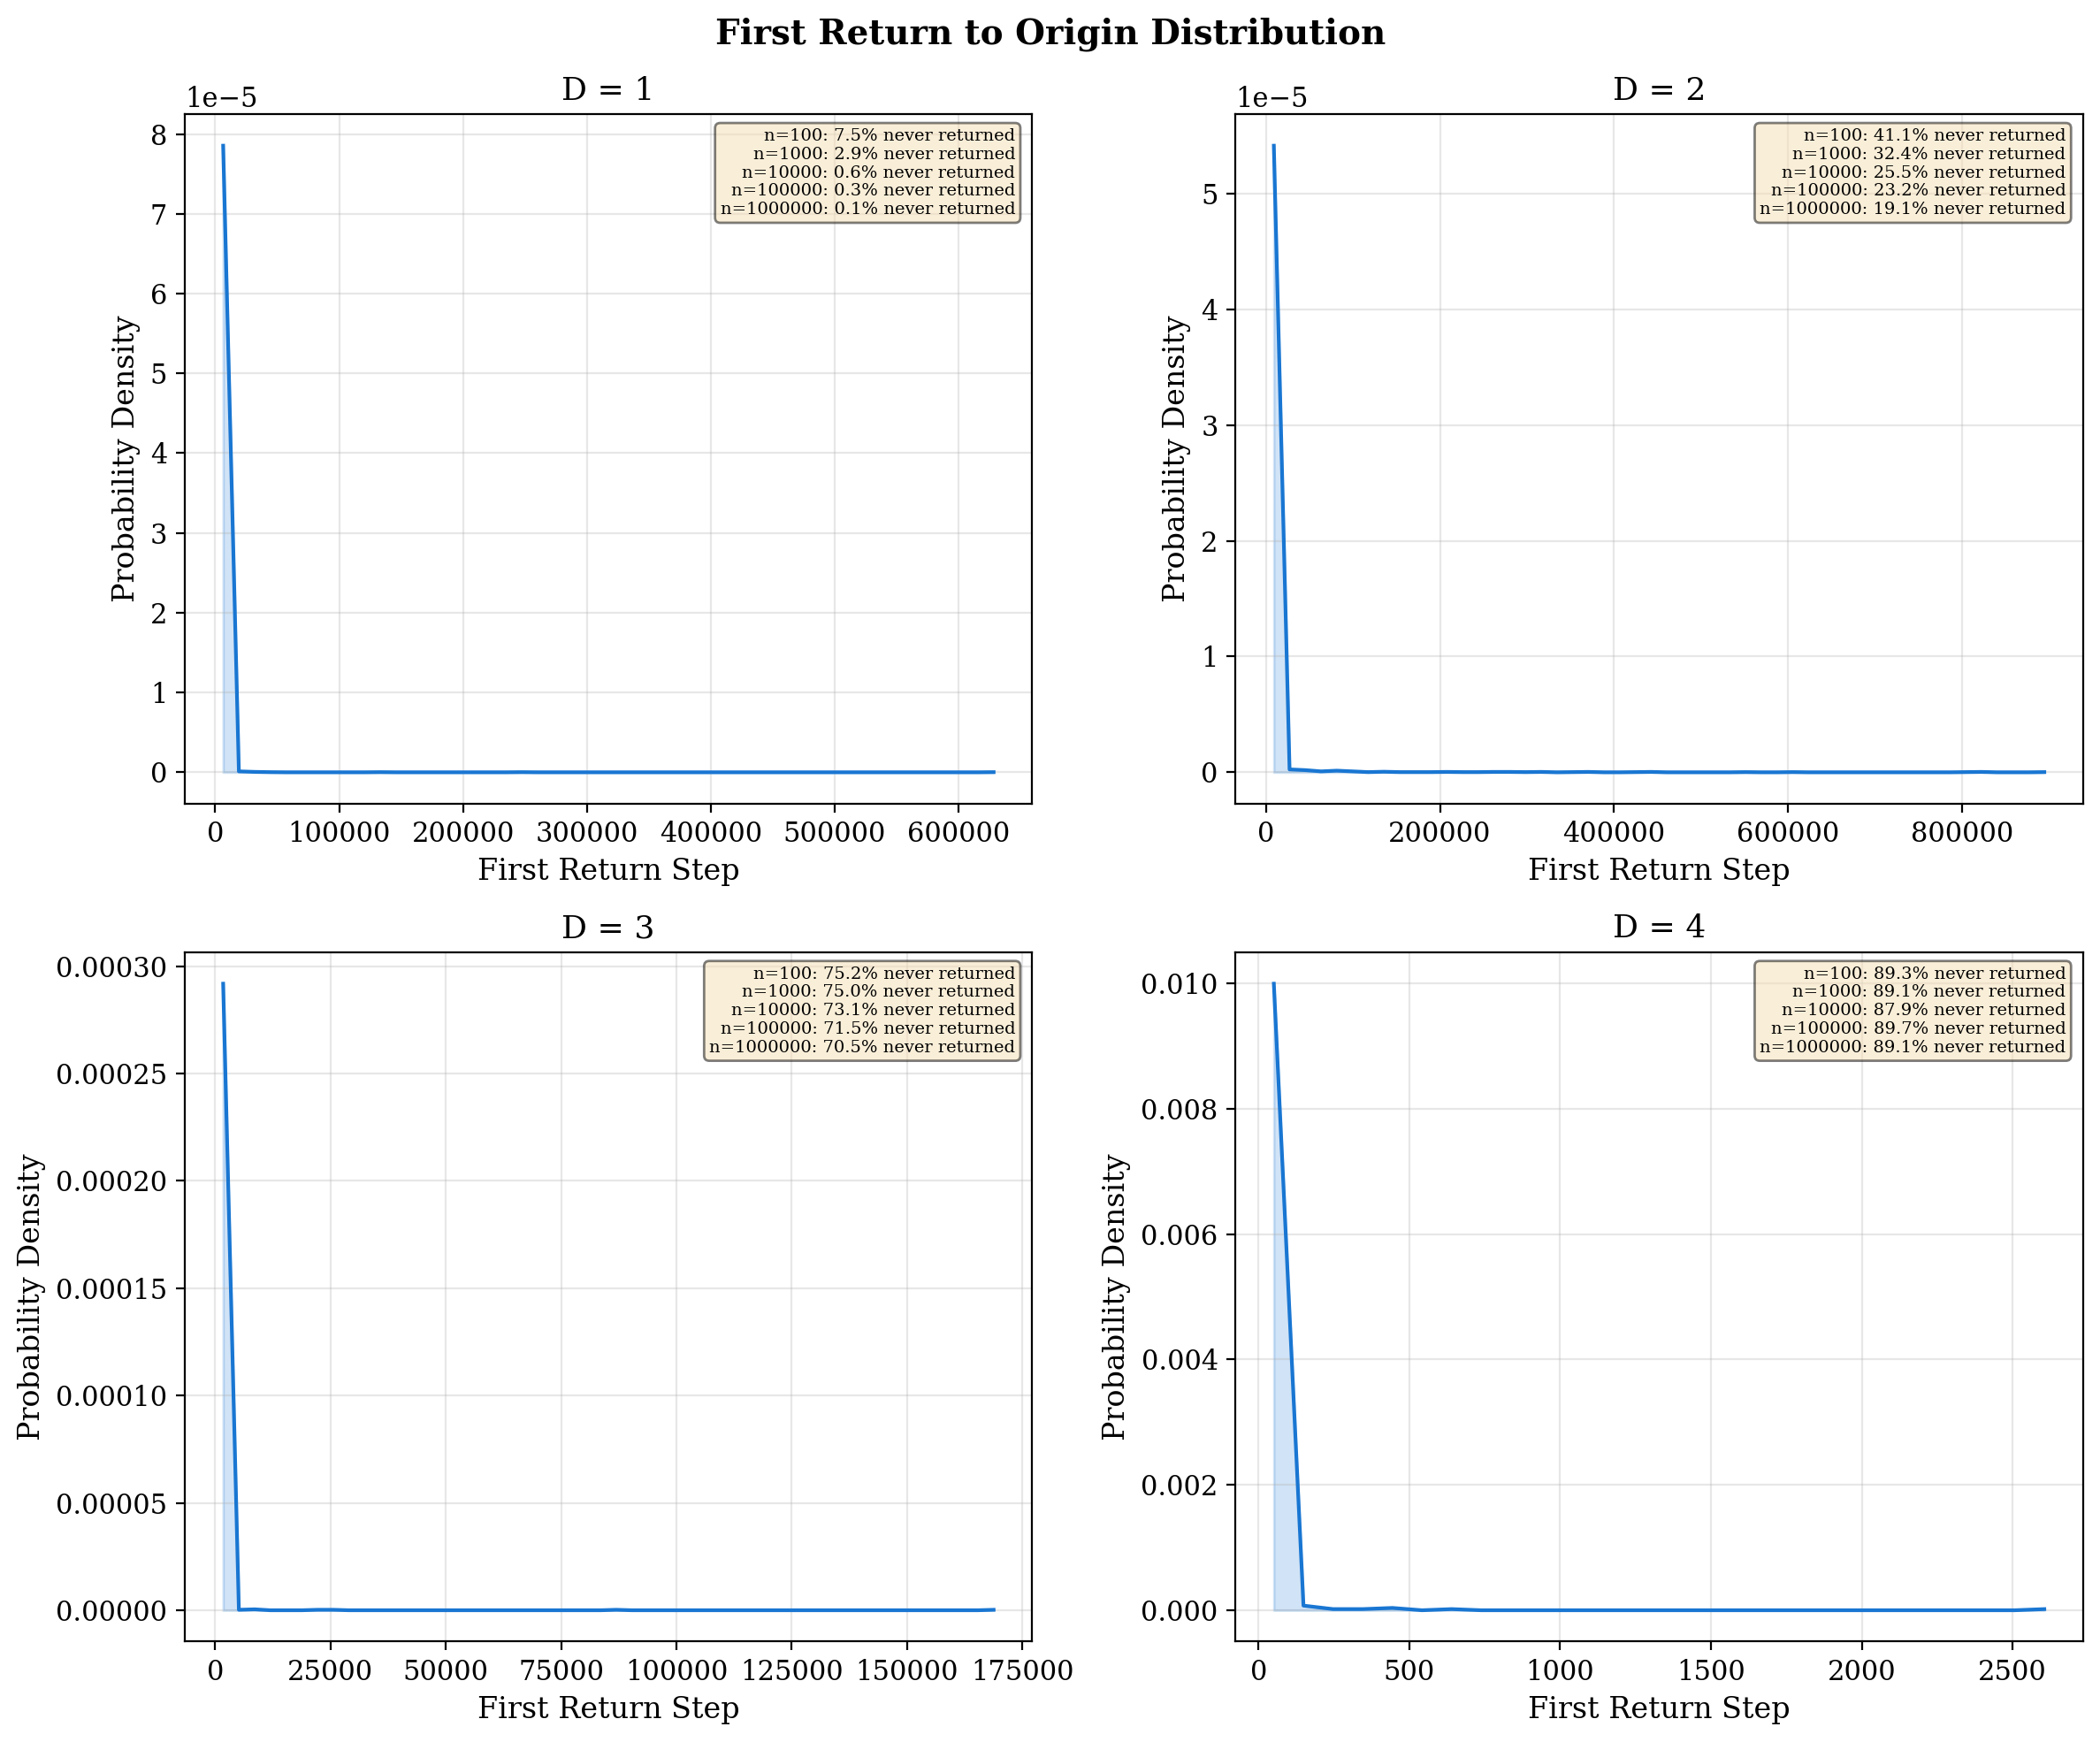
\includegraphics[width=0.85\textwidth]{return_to_origin.png}
  \caption{各維度的首次回到原點 step 數分佈}
  \label{fig:return}
\end{figure}

\subsubsection{回到原點次數分佈}

圖~\ref{fig:numret} 展示不同 $n$ 下回到原點的次數分佈。

\begin{figure}[H]
  \centering
  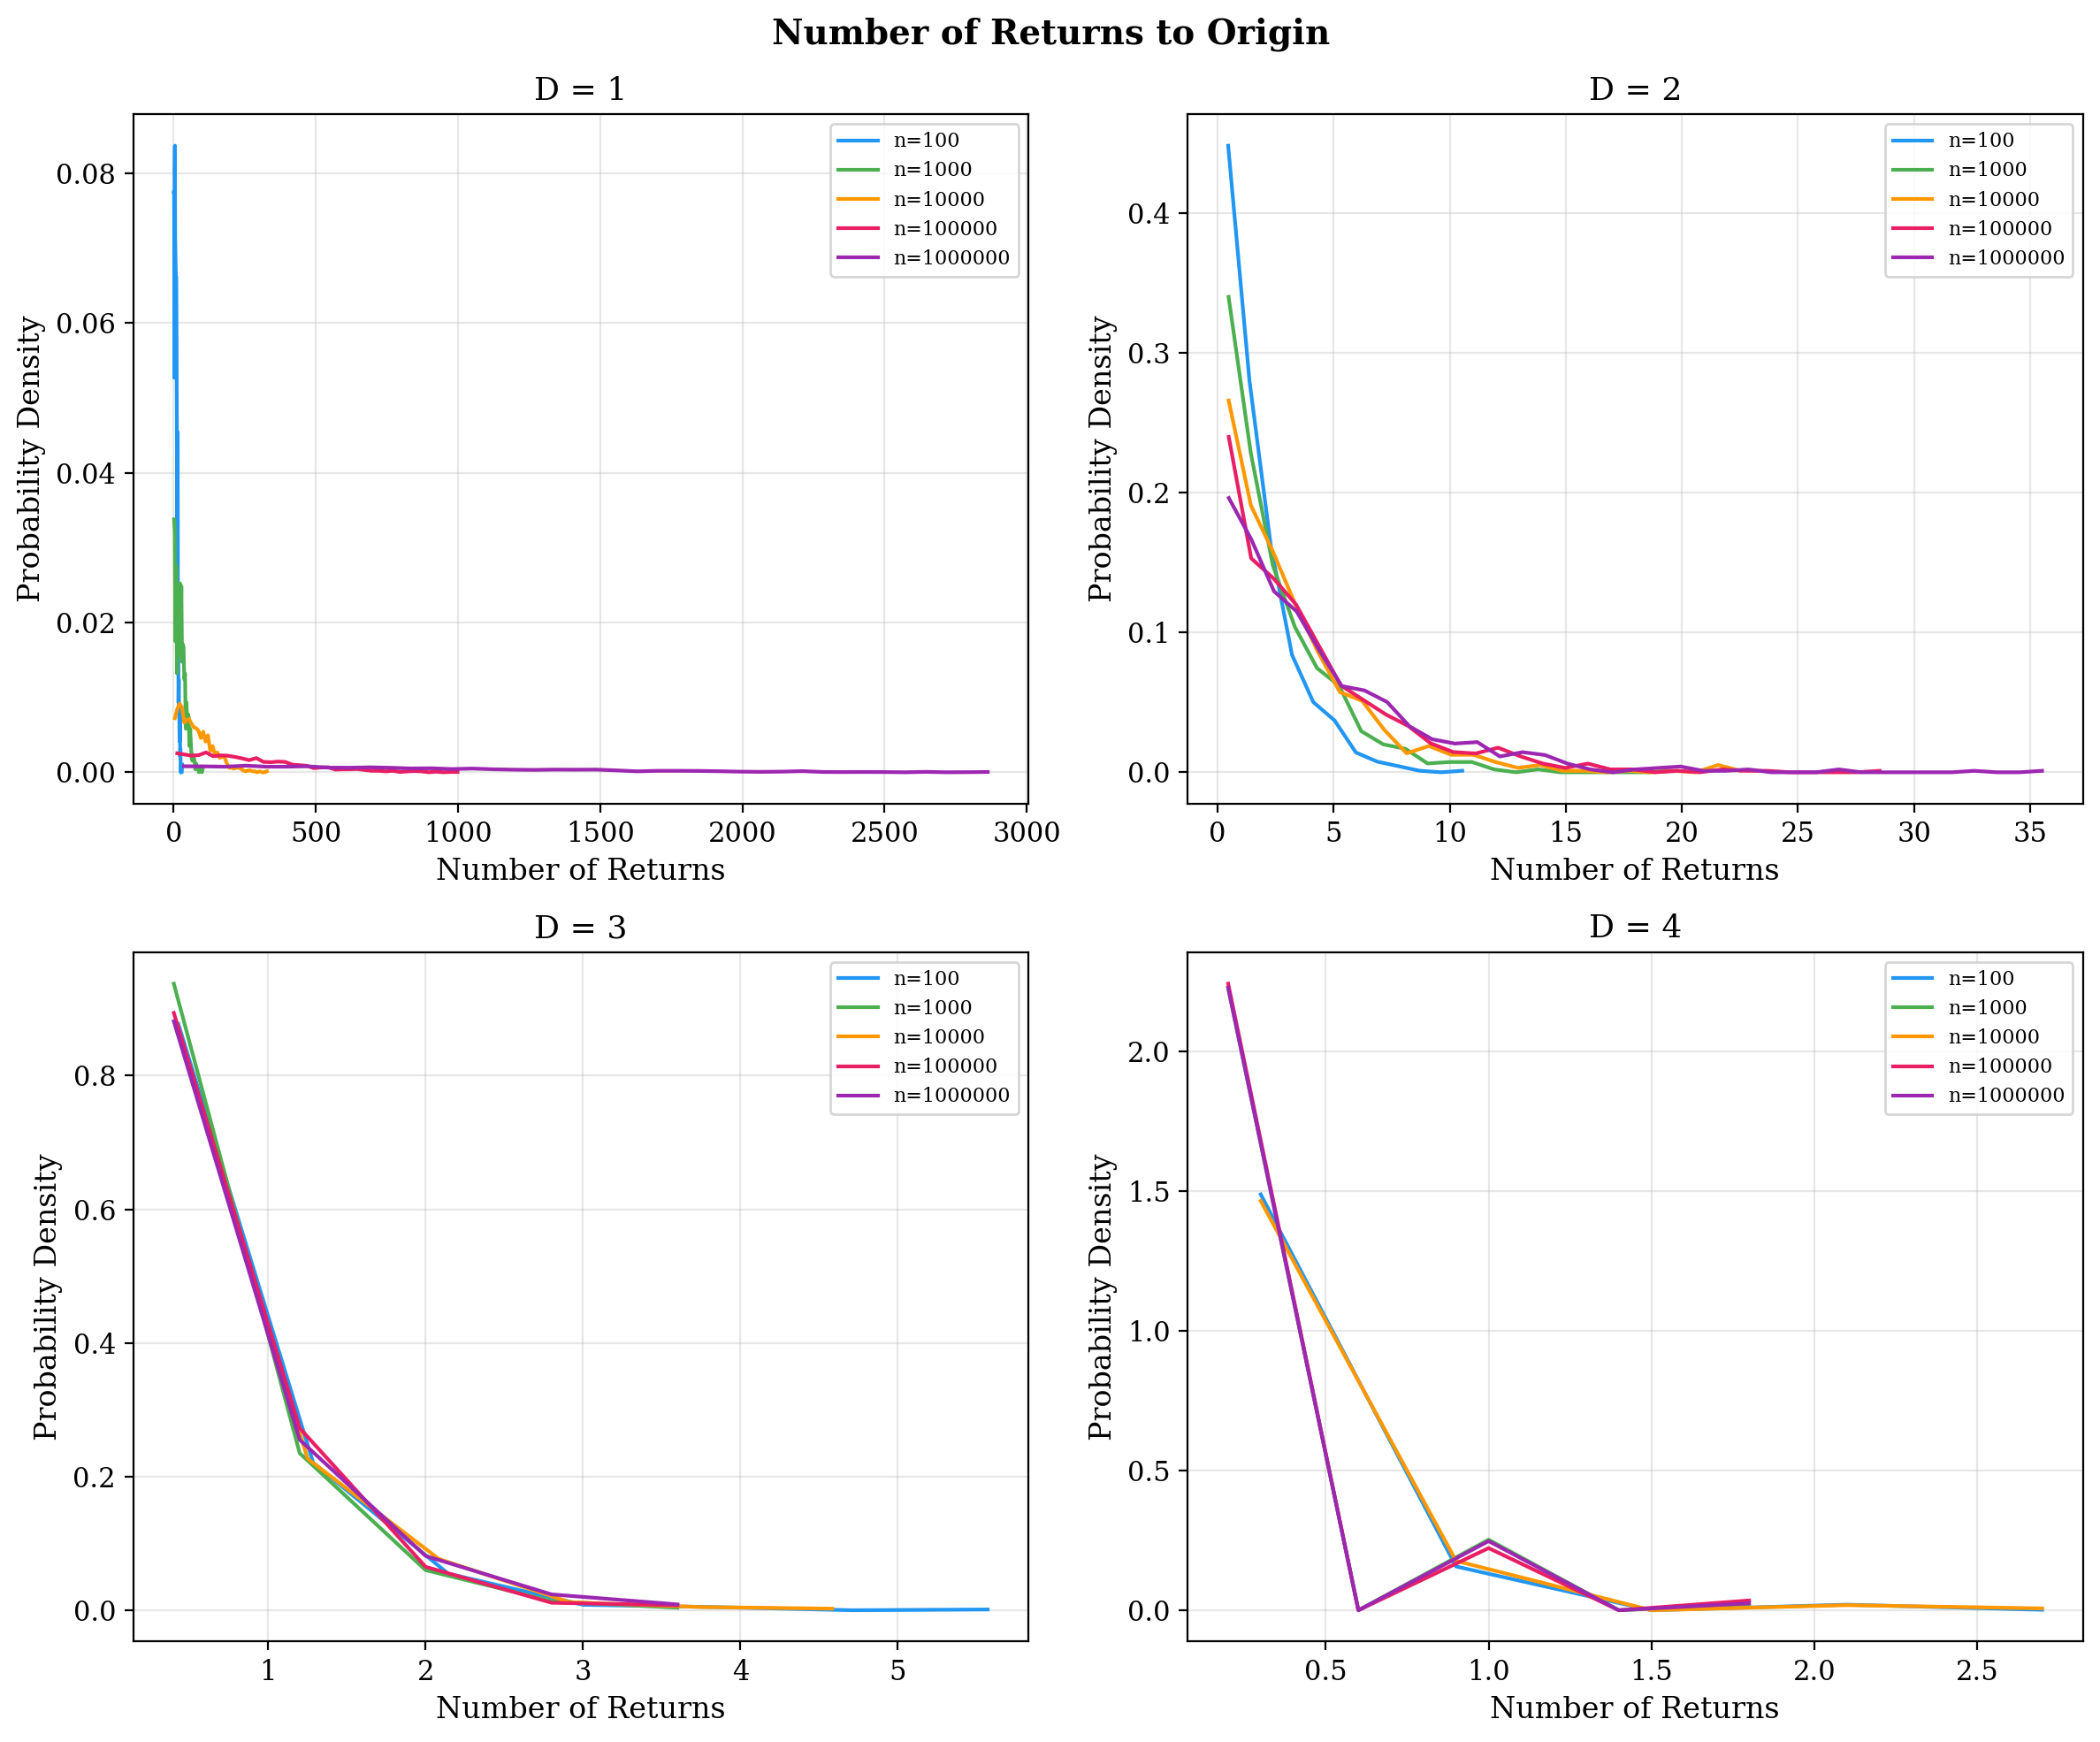
\includegraphics[width=0.85\textwidth]{num_returns.png}
  \caption{各維度的回到原點次數分佈}
  \label{fig:numret}
\end{figure}

\subsubsection{平均首次回到原點步數}

圖~\ref{fig:expret} 展示平均首次回到原點的步數與行走長度的關係。

\begin{figure}[H]
  \centering
  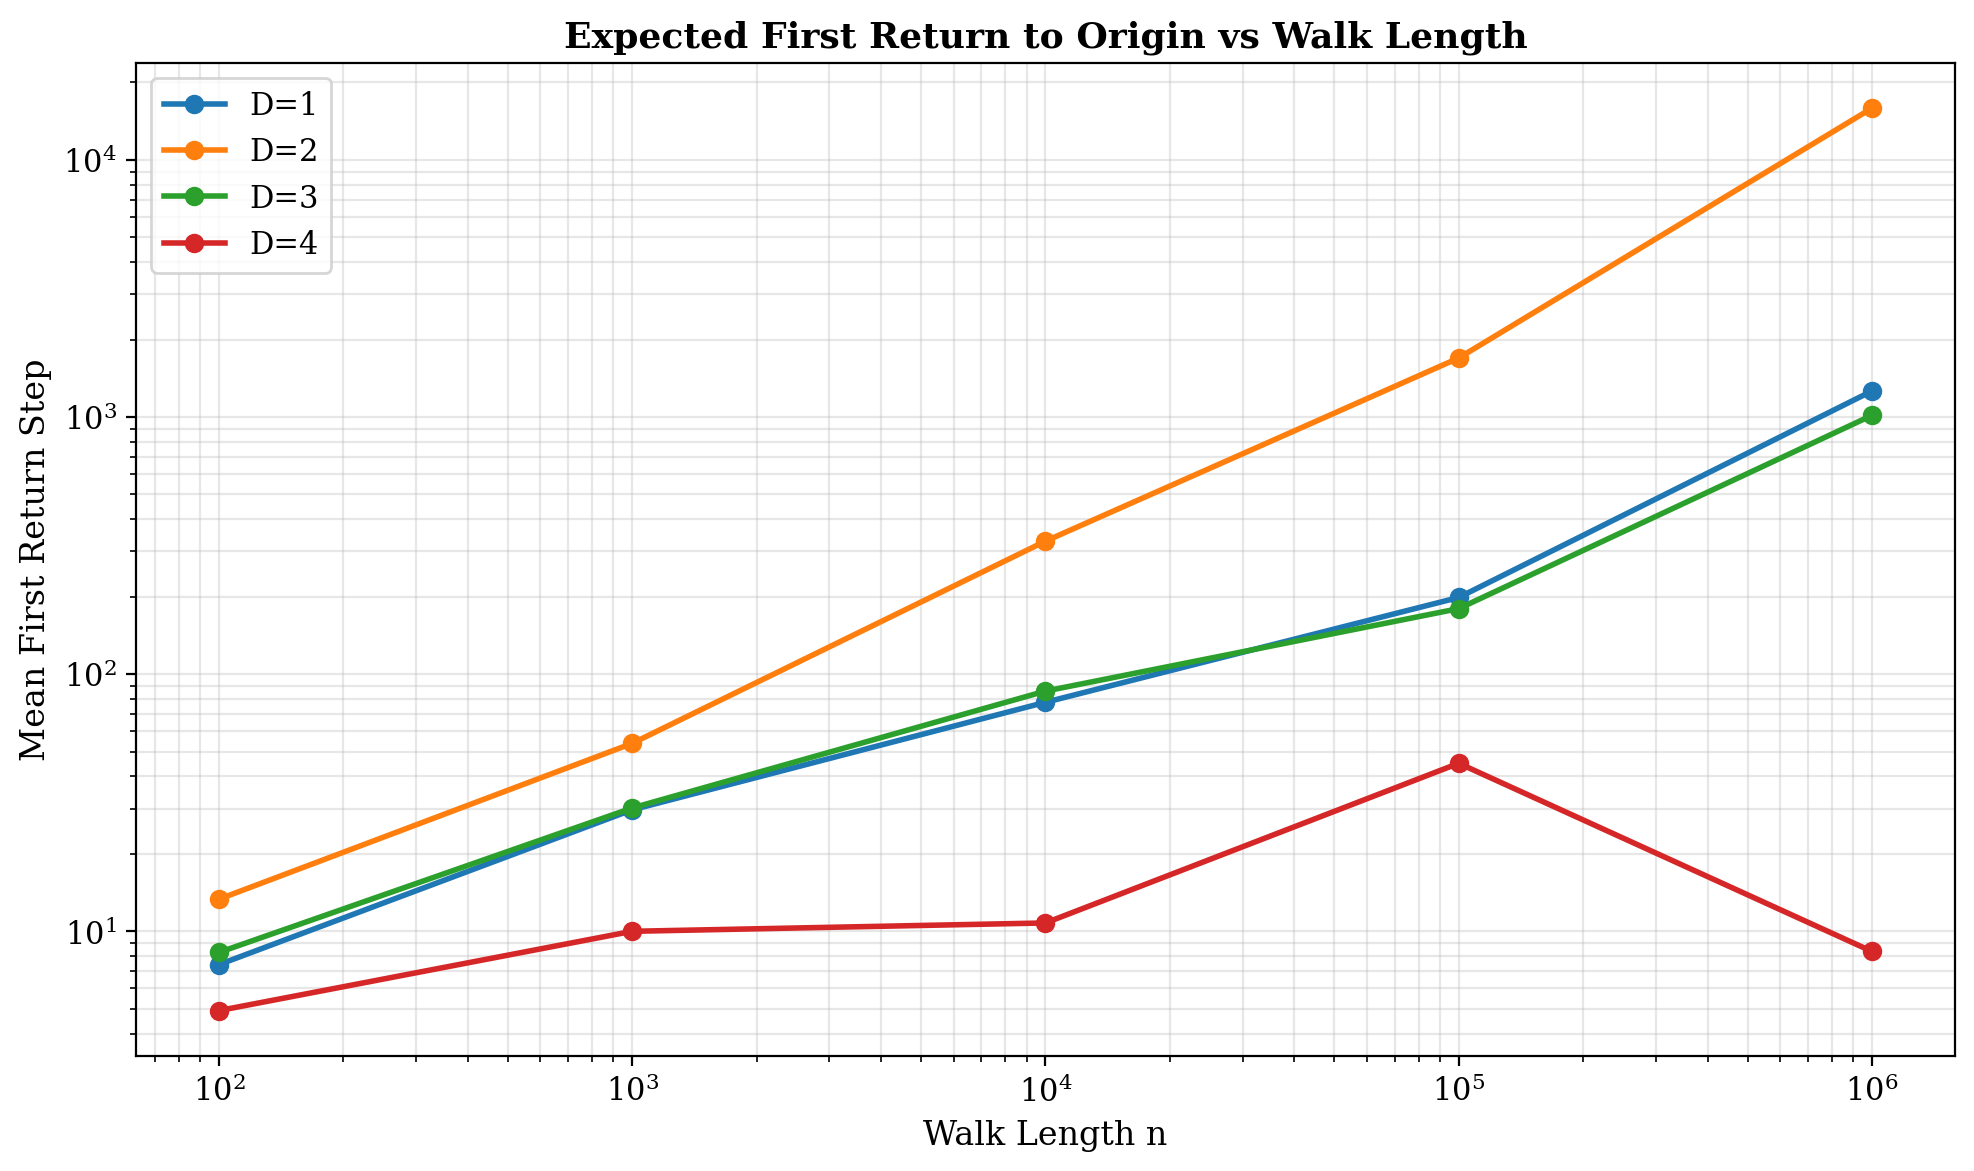
\includegraphics[width=0.7\textwidth]{expected_return.png}
  \caption{平均首次回到原點步數 vs 行走長度}
  \label{fig:expret}
\end{figure}

根據 \textbf{Pólya's Recurrence Theorem}：
\begin{itemize}[nosep]
  \item $D = 1, 2$：隨機行走是 \textbf{recurrent} 的，粒子以機率 1 回到原點
  \item $D \geq 3$：隨機行走是 \textbf{transient} 的，
        回到原點的機率 $P_{\text{return}} < 1$
\end{itemize}

具體而言，$D=3$ 時回到原點的機率約為 $P_3 \approx 0.3405$，
$D=4$ 時更低。從模擬結果可以清楚觀察到，
高維度下有更大比例的行走從未回到原點。

對於 $D \geq 3$ 無法回到原點的情況，我們的模擬數據提供了
首次回到原點期望步數的 lower bound。

\subsection{1D 專屬實驗：$m/n$ 分佈（Arcsine Law）}

定義：
\begin{align}
  n_- &= \text{粒子在負半軸的步數} \\
  n_0 &= \text{粒子在原點的步數} \\
  n_+ &= \text{粒子在正半軸的步數} \\
  m   &= \tfrac{1}{2} n_0 + \max(n_-, n_+)
\end{align}

圖~\ref{fig:mn} 展示 $m/n$ 的分佈，並與理論的 arcsine 分佈
$f(x) = \frac{1}{\pi\sqrt{x(1-x)}}$ 比較。

\begin{figure}[H]
  \centering
  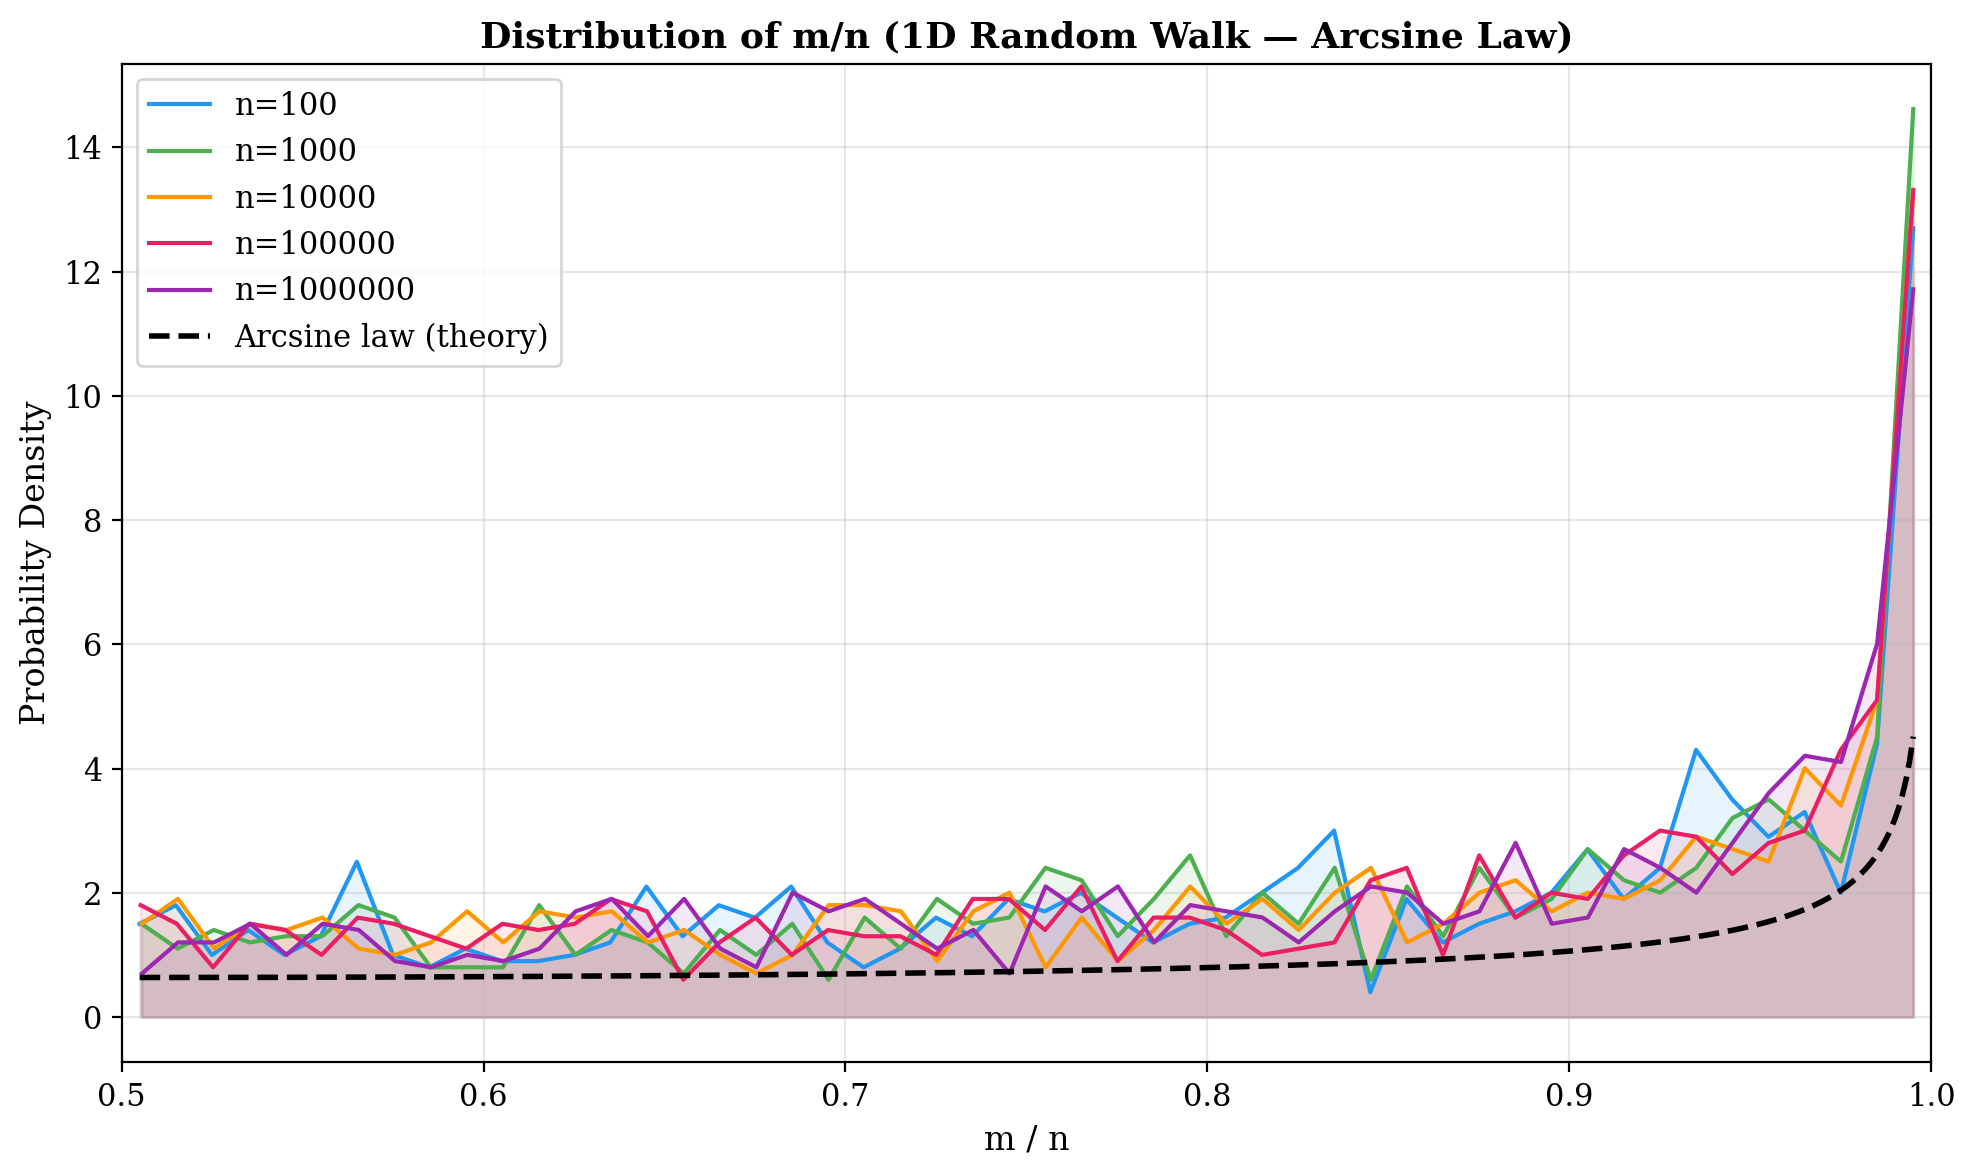
\includegraphics[width=0.85\textwidth]{m_over_n.png}
  \caption{1D Random Walk 的 $m/n$ 分佈與 arcsine law}
  \label{fig:mn}
\end{figure}

觀察與討論：
\begin{itemize}[nosep]
  \item $m/n$ 的分佈確實趨近於 arcsine 分佈，
        $n$ 越大擬合越好
  \item Arcsine 分佈在 $x = 0.5$ 和 $x = 1.0$ 附近有較高的密度，
        代表粒子傾向於「大部分時間」待在同一側，
        而非均勻分配正負半軸的時間
  \item 這個反直覺的結果是 random walk 理論中著名的 \textbf{arcsine law}，
        與 martingale 理論密切相關
\end{itemize}

% ╔═══════════════════════════════════════════════════════════╗
% ║  4. 結論                                                  ║
% ╚═══════════════════════════════════════════════════════════╝
\section{結論}

本報告透過大規模數值模擬，驗證了 random walk 的多項重要理論性質：
\begin{enumerate}[nosep]
  \item \textbf{距離 Scaling}：$\mathbb{E}[\|\mathbf{x}\|] \propto \sqrt{n}$，
        對所有維度成立
  \item \textbf{Symmetry}：各 section 的停留比例接近均勻
  \item \textbf{Pólya's Recurrence Theorem}：$D \leq 2$ 時 recurrent，$D \geq 3$ 時 transient
  \item \textbf{Arcsine Law}：1D random walk 的 $m/n$ 分佈服從 arcsine 分佈
\end{enumerate}

模擬結果與理論預測高度一致，
驗證了我們的實作正確性與統計分析方法的有效性。

% ╔═══════════════════════════════════════════════════════════╗
% ║  References                                               ║
% ╚═══════════════════════════════════════════════════════════╝
\begin{thebibliography}{9}
  \bibitem{grinstead}
    C.~M. Grinstead and J.~L. Snell,
    \textit{Introduction to Probability},
    Chapter 12: Random Walks.

  \bibitem{polya}
    G.~Pólya,
    ``Über eine Aufgabe der Wahrscheinlichkeitsrechnung betreffend die Irrfahrt im Straßennetz,''
    \textit{Mathematische Annalen}, vol.~84, pp.~149--160, 1921.

  \bibitem{feller}
    W.~Feller,
    \textit{An Introduction to Probability Theory and Its Applications},
    Vol.~1, Chapter III: Fluctuations in Coin Tossing and Random Walks.
\end{thebibliography}

\end{CJK}
\end{document}
